\documentclass[11pt,a4paper]{article}

\usepackage[margin=1in]{geometry}
\usepackage{booktabs}
\usepackage{longtable}
\usepackage{array}
\usepackage{tabularx}
\usepackage{hyperref}
\usepackage{xcolor}
\usepackage{enumitem}
\usepackage{fancyhdr}
\usepackage{titlesec}
\usepackage{microtype}
\usepackage{tcolorbox}
\usepackage{tikz}
\usetikzlibrary{positioning}
\usepackage{caption}
\usepackage{setspace}
\usepackage{amsmath}
\usepackage[T1]{fontenc}
\usepackage[utf8]{inputenc}

\hypersetup{
  colorlinks=true,
  linkcolor=blue!50!black,
  urlcolor=blue!50!black,
  pdftitle={N2S Evidence Grounding Lab --- Progress Notes},
  pdfauthor={CXR evidence-grounding lab}
}

\definecolor{okgreen}{HTML}{166534}
\definecolor{warnamber}{HTML}{92400E}
\definecolor{contrared}{HTML}{7C2D12}
\definecolor{muted}{HTML}{57534E}
\definecolor{paper}{HTML}{FFFDF8}

\pagestyle{fancy}
\fancyhf{}
\fancyhead[L]{\small N2S Evidence Grounding Lab}
\fancyhead[R]{\small Progress notes --- 25 Aug 2026}
\fancyfoot[C]{\thepage}
\renewcommand{\headrulewidth}{0.3pt}

\titleformat{\section}{\large\bfseries}{\thesection}{0.6em}{}
\titleformat{\subsection}{\normalsize\bfseries}{\thesubsection}{0.6em}{}

\setlist[itemize]{leftmargin=1.4em,itemsep=0.25em,topsep=0.4em}
\setlist[enumerate]{leftmargin=1.4em,itemsep=0.25em,topsep=0.4em}

\newcommand{\pred}{\texttt{FIRST\_LINE\_THERAPY\_FAILED}}
\newcommand{\sat}{\textsc{Satisfied}}
\newcommand{\nsat}{\textsc{NotSatisfied}}
\newcommand{\unc}{\textsc{Uncertain}}
\newcommand{\con}{\textsc{Contradiction}}
\newcommand{\rev}{\textsc{Review}}

\newcolumntype{L}[1]{>{\raggedright\arraybackslash}p{#1}}
\newcolumntype{Y}{>{\raggedright\arraybackslash}X}

\begin{document}

\begin{center}
{\LARGE\bfseries Neural-to-Symbolic Evidence Grounding}\\[0.35em]
{\large Progress notes}\\[0.8em]
{\color{muted} Working lab notebook, not a paper and not a claim of clinical validity.}\\[0.6em]
24~August~2026 \quad$\cdot$\quad M1--M3 and Phase~1--11 frozen\\[0.3em]
{\small Isolated lab: \texttt{staging/cxr-evidence-grounding-lab/}
\quad UI: \url{http://127.0.0.1:8253/}}
\end{center}

\vspace{0.6em}
\begin{tcolorbox}[colback=paper,colframe=black!20,boxrule=0.4pt,arc=1pt,left=8pt,right=8pt,top=6pt,bottom=6pt]
\textbf{Status of this document.}
M1--M3 through Phase~1--11 are frozen (A--D; verify/\rev; safety stack; BC\_E1 rep-eng Ph9--11 + explorer \texttt{:8256}).
Working lab notebook, not a paper and not a claim of clinical validity.
UIs: \texttt{:8253} M1, \texttt{:8254} A--D, \texttt{:8255} Phase~5--7 safety stack.
Rebuild with \texttt{latexmk -pdf progress-notes.tex} from the \texttt{notes/} directory.
\end{tcolorbox}

\tableofcontents
\vspace{0.8em}

\section{The question}

\begin{quote}
\textit{Can a system reliably determine whether evidence expressed in natural language satisfies a formally defined condition?}
\end{quote}

Milestone~1 was deliberately tiny: \textbf{one} formal condition, \textbf{twenty} hand-authored oncology-note snippets, and a \textbf{direct-LLM baseline} so the structured pipeline could be compared rather than merely demonstrated.

Accuracy was \emph{not} the objective. Version~1 succeeds if the neural-to-symbolic boundary is \textbf{observable}---same requirement, different wording, extraction, atoms, rule---and we can mark succeed / fail / uncertain / contradiction.

\paragraph{Hard constraints.}
The lab does not modify CXR production (\texttt{claim\_analysis\_tools}, Claim Studio, rehearsal UI).
It does not add extra predicates, Qdrant, Archetypes, or Next.js.
Mock-mode keyword extraction is for inspecting the symbolic path; it is \textbf{not} a research result.
The direct-LLM baseline is never skipped on live runs.
Gold labels are shown in the UI and are \textbf{not} sent to the model.

\paragraph{Model.}
Local Ollama \texttt{llama3:8b-instruct-q4\_0} at \texttt{127.0.0.1:11434}.

\section{System under test}

Two paths, same notes, same predicate.

\vspace{0.6em}
\begin{center}
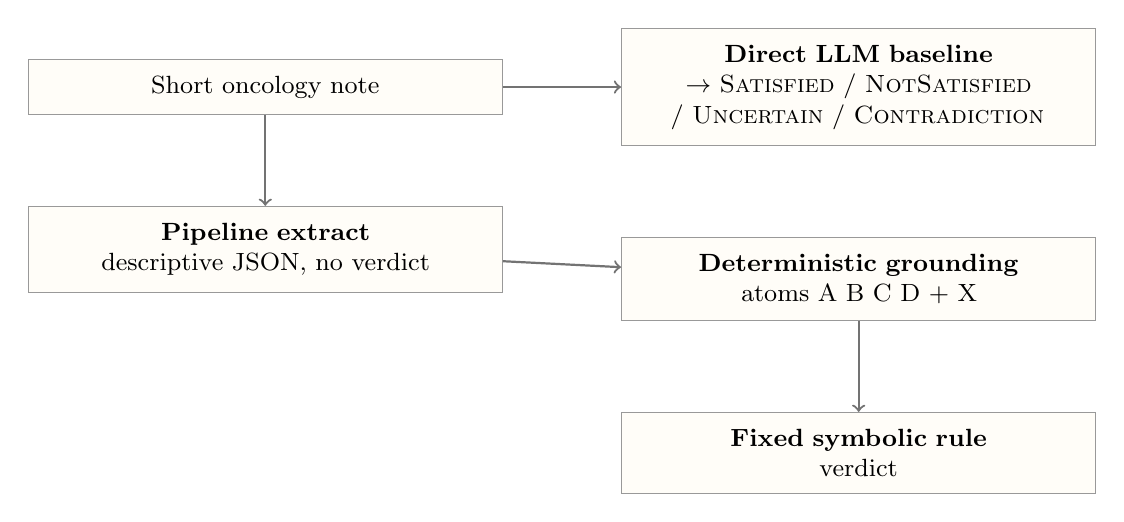
\begin{tikzpicture}[
  font=\small,
  box/.style={draw=black!40, fill=paper, align=center, inner sep=6pt, text width=5.6cm},
  arr/.style={->, thick, black!55}
]
\node[box] (note) {Short oncology note};
\node[box, right=1.5cm of note] (base) {\textbf{Direct LLM baseline}\\$\rightarrow$ \sat{} / \nsat{}\\ / \unc{} / \con};
\node[box, below=1.15cm of note] (ex) {\textbf{Pipeline extract}\\descriptive JSON, no verdict};
\node[box, below=1.15cm of base] (gnd) {\textbf{Deterministic grounding}\\atoms A B C D + X};
\node[box, below=1.15cm of gnd] (rule) {\textbf{Fixed symbolic rule}\\verdict};
\draw[arr] (note) -- (base);
\draw[arr] (note) -- (ex);
\draw[arr] (ex) -- (gnd);
\draw[arr] (gnd) -- (rule);
\end{tikzpicture}
\end{center}

\paragraph{Predicate.} \pred{} holds iff all of:

\begin{center}
\begin{tabular}{@{}c l L{10.6cm}@{}}
\toprule
Atom & Name & Meaning \\
\midrule
A & first-line identified & A first-line (front-line / 1L) systemic therapy is identified, explicitly or by conventional implication. \\
B & first-line administered & That therapy was given or attempted, not merely planned. \\
C & failure event & Progression, non-response, clinician statement of failure/refractory disease, or discontinuation for intolerance without a plan to resume. \\
D & failure of first-line & The failure event is of that first-line regimen (not only a later line; not completed adjuvant therapy with NED). \\
X & contradiction & Mutually incompatible claims about A--D. \\
\bottomrule
\end{tabular}
\end{center}

\paragraph{Rule (unchanged across milestones).}
\con{} if X;
else \nsat{} if any of A, B, C, D is false;
else \unc{} if any is unknown;
else \sat{} if $A \land B \land C \land D$.

\paragraph{UI marks.}
\texttt{P+}/\texttt{P$-$} = pipeline matches / misses \textbf{gold}.
\texttt{B+}/\texttt{B$-$} = direct LLM matches / misses gold.
These are not ``the predicate is true.''

\section{Evaluation set}

Twenty synthetic snippets. Four wording categories, four cases each. Gold is a four-way label, not yes/no.
Full text lives in \texttt{data/cases.json}. The \texttt{why} field is the gold rationale (shown in the UI, not sent to the model).

\subsection{Explicit (E) --- the note almost says it}

\begin{tabularx}{\textwidth}{@{}c l Y@{}}
\toprule
ID & Gold & Why included \\
\midrule
E1 & \sat & Named first-line + explicit progression. \\
E2 & \sat & Stopped for intolerance (counts as line failure). \\
E3 & \nsat & Ongoing first-line with response. \\
E4 & \nsat & First-line only planned; never given. \\
\bottomrule
\end{tabularx}

\subsection{Implicit (I) --- you have to infer it}

\begin{tabularx}{\textwidth}{@{}c l Y@{}}
\toprule
ID & Gold & Why included \\
\midrule
I1 & \sat & New lesions $\rightarrow$ switch to second-line (never says ``failed''). \\
I2 & \sat & ``Platinum-refractory'' as conventional 1L failure language. \\
I3 & \nsat & Future plan only. \\
I4 & \nsat & Completed adjuvant + NED $\neq$ metastatic first-line failure. \\
\bottomrule
\end{tabularx}

\subsection{Temporal (T) --- order in time matters}

\begin{tabularx}{\textwidth}{@{}c l Y@{}}
\toprule
ID & Gold & Why included \\
\midrule
T1 & \sat & Initial response, then later progression on 1L. \\
T2 & \nsat & Cycle 1 day 2; too early. \\
T3 & \sat & Response then progression; now on second-line. \\
T4 & \nsat & Hold for neutropenia with plan to resume. \\
\bottomrule
\end{tabularx}

\subsection{Uncertain (U) --- incomplete or mixed}

\begin{tabularx}{\textwidth}{@{}c l Y@{}}
\toprule
ID & Gold & Why included \\
\midrule
U1 & \unc & Possible progression; awaiting confirmatory scan. \\
U2 & \unc & May have received platinum; outcome unknown. \\
U3 & \unc & Mixed response. \\
U4 & \unc & Unclear whether metastatic 1L or adjuvant; no clear progression. \\
\bottomrule
\end{tabularx}

\subsection{Conflicting (C) --- two parts of the note disagree}

\begin{tabularx}{\textwidth}{@{}c l Y@{}}
\toprule
ID & Gold & Why included \\
\midrule
C1 & \con & Same-day assessment ``failed'' vs addendum ``continue 1L with SD''. \\
C2 & \con & ``Never received systemic therapy'' vs six cycles then progression. \\
C3 & \con & Referring ``failed 1L'' vs chart review ``never started''. \\
C4 & \con & Same regimen: ``progressed'' vs later ``excellent ongoing response''. \\
\bottomrule
\end{tabularx}

\section{Journey of the evaluation}

\subsection{Milestone 1 --- make the boundary visible}

\paragraph{Intervention.}
Isolated lab, one predicate, 20~cases, two paths, UI on port 8253.

\paragraph{Live 20-case run}
(\texttt{artifacts/live-m1-before-contradiction.json}):

\begin{center}
\begin{tabular}{@{}l r@{}}
\toprule
Path & Match gold \\
\midrule
Pipeline & \textbf{13/20} \\
Direct LLM & \textbf{12/20} \\
Disagree with each other & I2, T2, U1, U3, U4 \\
\bottomrule
\end{tabular}
\end{center}

By category (pipeline / baseline correct): explicit 4/4 and 4/4; implicit 3/4 and 4/4; temporal 4/4 and 3/4; uncertain 2/4 and 1/4; \textbf{conflicting 0/4 and 0/4}.

\paragraph{What we learned.}
\begin{itemize}
  \item Explicit cases are easy for both. Structure is not ``doing extra work'' there.
  \item \textbf{I2:} baseline \sat{} (correct); pipeline missed at \textbf{extraction} (implicit platinum-refractory $\rightarrow$ B false). The fail is not the rule. Decision: do not chase I2 accuracy.
  \item \textbf{T2, U1, U3:} pipeline closer to gold; baseline over-called \sat{} or \nsat.
  \item \textbf{C1--C4:} both missed all four. On C1 the baseline \emph{described} the addendum conflict, then still emitted \nsat.
\end{itemize}

The interesting failure was contradiction information \textbf{recognized in language and dropped before the rule}.

\subsection{Milestone 2 --- first-class contradiction}

\paragraph{Intervention.}
Extractor must always fill \texttt{contradiction.present} = true (two incompatible spans) or false (explicit none).
Grounding sets \textbf{X} from that field.
\textbf{Rule unchanged.}

\paragraph{Finding worth writing.}
The LLM can notice contradiction in prose and still not emit \con{} as a verdict.
Putting two spans on the interface lets the symbolic rule fire.

Live pattern on C (from \texttt{artifacts/live-c1-c4.json} and the M2 full run):

\begin{center}
\begin{tabular}{@{}c l l@{}}
\toprule
Case & Pipeline & Direct LLM \\
\midrule
C1 & \con & \nsat{} (rationale still describes the conflict) \\
C2 & \con & \sat \\
C3 & \con & \nsat \\
C4 & \nsat & \nsat{} (\texttt{present=false}) \\
\bottomrule
\end{tabular}
\end{center}

Headline score stayed about \textbf{13/20 vs 12/20}. The \emph{kind} of error changed, not the leaderboard.

\paragraph{Cost of M2.}
\textbf{U4} (uncertain line of therapy) was called \con{} by the pipeline --- X over-fired on ``metastatic vs adjuvant?''

\paragraph{C4 left failing on purpose.}
It is not the same \emph{class} as C1--C3 (surface incompatible records / addendum).
Progressed-at-$T_1$ vs excellent-response-at-$T_2$ on the same regimen might be conflict \emph{or} clinical course.
Stretching span extraction to ``fix'' C4 would hide that class.
We do not interpret the miss as proof that a temporal-reasoning module is missing.

\subsection{Milestone 2.1 --- X is not uncertainty}

\paragraph{Intervention.}
Prompt + grounding: unresolved which-line / mixed / pending $\rightarrow$ uncertainty, \textbf{not} X.
Do \textbf{not} try to make C4 pass.

Live slice (\texttt{artifacts/live-m2.1-c-u4.json}):

\begin{center}
\begin{tabular}{@{}c l l l@{}}
\toprule
Case & Pipeline & Direct LLM & X \\
\midrule
C1 & \con & \nsat & true \\
C2 & \con & \sat & true \\
C3 & \con & \nsat & true \\
C4 & \nsat & \nsat & false (still the hard miss) \\
U4 & \nsat & \unc & \textbf{false} (no longer \con) \\
\bottomrule
\end{tabular}
\end{center}

U4 hygiene succeeded (X off).
U4 was \textbf{not} gold-correct this run (gold \unc; pipeline \nsat{} from atoms).
That is leftover uncertainty calibration, not a reason to reopen C4.

\subsection{Milestone 3 --- first-class uncertainty}

\paragraph{Intervention.}
Extractor must always fill \texttt{uncertainty.present} = true (one cue + why) or false (explicit none).
Grounding keeps implicated A--D atoms \textbf{unknown}.
\textbf{Rule unchanged} (\unc{} still comes from unknown atoms, not a new U atom in the formula).
Do not rewrite A--D or X.

Live slice (\texttt{artifacts/live-m3-u-c.json}): U1--U4 + C1--C4.

\begin{center}
\begin{tabular}{@{}c l l l l@{}}
\toprule
ID & Pipeline & Baseline & \texttt{U.present} & X \\
\midrule
U1 & \unc & \sat & true (pending) & false \\
U2 & \unc & \nsat & true (unknown outcome) & false \\
U3 & \unc & \nsat & true & false \\
U4 & \unc & \unc & true (unresolved line) & \textbf{false} \\
C1 & \con & \nsat & false & true \\
C2 & \con & \sat & false & true \\
C3 & \con & \nsat & false & true \\
C4 & \nsat & \nsat & false & false (still miss) \\
\bottomrule
\end{tabular}
\end{center}

\paragraph{Finding.}
Same pattern as M2, but \textbf{do not treat U1--U4 as one M3 win.}
U1/U3 were often already \unc{} from unknown atoms before this field existed.
The distinctive M3 save is \textbf{U2/U4} no longer collapsing to \nsat{} once \texttt{uncertainty.present} sits on the extract$\rightarrow$ground contract.
The baseline still over-commits on U1--U3 (\sat{} / \nsat); on this run it matched gold on U4.
C1--C3 still \con{} vs baseline not; C4 left in the failure set; U4 X stayed false.

\paragraph{Hypothesis (lab scale; not a new architecture).}
Reliable neuro-symbolic \emph{verdicts here} depend not only on extracting facts, but on preserving semantic states such as uncertainty and contradiction across the neural-to-symbolic boundary.
Scope: one predicate, twenty notes, one local 8B model. The score (about 13/20 vs 12/20) is not the result.

\section{What M1--M3 demonstrated (frozen)}

The same underlying pattern appeared twice, and the rule engine did not change:

\begin{center}
\begin{tabularx}{\textwidth}{@{}l Y Y@{}}
\toprule
State & Recognized in language & Preserved only when explicit at the N2S boundary \\
\midrule
Contradiction & Baseline can \emph{describe} conflict (C1) & C1--C3: two spans $\rightarrow$ X $\rightarrow$ \con \\
Uncertainty & Baseline can see insufficient evidence & U2/U4: cue+why $\rightarrow$ unknown atoms $\rightarrow$ \unc \\
\bottomrule
\end{tabularx}
\end{center}

\paragraph{What each slice is for.}
\begin{itemize}
  \item \textbf{C1--C3} show that an explicit contradiction state prevents conflict from being flattened into an ordinary verdict.
  \item \textbf{U2/U4} show that an explicit uncertainty state prevents ambiguous evidence from being flattened into \sat{} or \nsat.
  \item \textbf{U1/U3} already often came out \unc{} from unknown atoms; they are supporting cases, not the M3 increment.
  \item The \textbf{direct LLM still over-commits} on U1--U3.
  \item \textbf{C4} remains a deliberately unresolved case: span-pair X is not enough when the apparent conflict depends on regimen identity and time. Gold$=$\con{} is a design choice; the miss is the scientific object. This does \emph{not} yet prove that a temporal reasoner is required---only that richer output fields do not cover that class.
\end{itemize}

\paragraph{Sentence the leftover buys.}
Explicit state representation solves some boundary failures, but not failures that require deeper temporal or contextual reconciliation.
That distinction keeps the result from becoming trivial.

\paragraph{What we are not claiming.}
Not production CXR.
Not that more extract fields will keep fixing errors.
Not that the pattern holds beyond this 20-note, one-predicate, one-model lab.
A larger controlled set is the \emph{next experiment after this write-up}, not the next field.

\section{What we are doing next (Phase~1, in plain language)}

M1--M3 are frozen. The next optional experiment does \textbf{not} add new medical rules or rebuild CXR.

\paragraph{Everyday picture.}
Imagine a careful reader who writes notes about a patient chart, then circles one final answer.
Sometimes the notes say ``these two sentences disagree,'' but the circled answer still looks like an ordinary yes/no.
We want to know: \textbf{at which step did the important idea get lost?}

\paragraph{Four places to look.}
\begin{enumerate}
  \item The written notes never notice the problem.
  \item The notes notice it, but the circled answer ignores it.
  \item The notes notice it, but our structured checklist drops it.
  \item The checklist is right, but our fixed rule still gets the answer wrong.
\end{enumerate}

\paragraph{Four ways we ask the same cases.}
We reuse only C1--C4 and U1--U4 (same gold labels; we still do not ``fix'' C4):
\begin{itemize}
  \item \textbf{A} --- ask for a final answer directly.
  \item \textbf{B} --- ask for free-text notes first, then a final answer from those notes.
  \item \textbf{C} --- use the existing structured pipeline (Milestone~3 style).
  \item \textbf{D} --- take the free-text notes, convert them into structure, then run the same rule.
\end{itemize}

\paragraph{What we will report.}
Not ``the score went up.'' We will count, when the answer is wrong, \textbf{how often each of the four places was the first place meaning disappeared.}

\paragraph{Safe to abandon.}
This Phase~1 code is optional and separate from Milestones~1--3.
If the direction is not useful, delete \texttt{run\_phase1\_diagnostic.py}, \texttt{n2s\_lab/phase1\_diagnostic.py}, and \texttt{artifacts/phase1-*.json}. The original lab keeps working.

\paragraph{Technical note (one sentence).}
Today's structured LLM calls ask for JSON and parse it; they are not hard-forced field-by-field constrained decoding.

\paragraph{First live Phase~1 numbers (same 8B model; C1--C4 + U1--U4).}
Match gold: direct answer A $=1/8$; notes-then-answer B $=3/8$; structured pipeline C $=7/8$; notes-then-structure D $=4/8$.
When the answer missed gold, the first-loss labels were roughly:
A --- almost all ``direct miss'';
B --- mix of ``notes noticed it but answer ignored it'' and ``notes never noticed it'';
C --- only C4 still missed (left unresolved on purpose);
D --- several times the notes had the idea but the structured form dropped it.
These counts are a first diagnostic snapshot, not a claim that the direction is finished.

\section{Phase~1 frozen interpretation (path comparison, not ``C wins'')}

\paragraph{What we freeze.}
Prompts for Conditions A--D, the eight case ids (C1--C4, U1--U4), gold labels, and the four first-loss stage labels.
We do \textbf{not} retune prompts after seeing Phase~1 misses, and we leave C4 unresolved by design.

\paragraph{How to read the path comparison.}
C looking strong on this slice is expected: the structured contract was shaped on the same failure types that appear in these eight notes.
That is a \textbf{test-set design risk}, not proof that structured extraction is generally best.
The scientifically interesting path is often \textbf{D}: free-text analysis already carries contradiction or uncertainty, then formalization drops it (\texttt{representation\_loss}).
Keep B's ``analysis$\rightarrow$answer mismatch'' separate from D's ``analysis$\rightarrow$structure loss''---they are different loci at the neural$\rightarrow$symbolic boundary.

\paragraph{Defensible claim (lab-scale, pending Phase~2).}
If the same drop-at-formalization pattern repeats across models and later across unseen wording, we have a research problem around \textbf{semantic preservation} at the neural$\rightarrow$symbolic interface.
If stronger models largely eliminate it, the Phase~1 pattern is more likely an engineering / capability issue for CXR tooling.

\section{Phase~2 --- cross-model panel (agreed next step)}

\paragraph{Protocol.}
Reuse the frozen A--D prompts and the same eight cases.
Rerun on a small local model panel with \textbf{no} per-model prompt tuning.
Compare whether D's \texttt{representation\_loss} (and B's analysis$\rightarrow$answer mismatch) repeats.

\paragraph{Local panel (no external API in this lab run).}
\begin{itemize}
  \item \texttt{llama3:8b-instruct-q4\_0} --- control (M1--M3 / Phase~1 reference); reuse existing Phase~1 artifact when present.
  \item \texttt{mistral:instruct} --- different family, similar size.
  \item \texttt{qwen2.5-coder:32b} --- stronger local model available on this machine (coder-tuned; still useful as a capacity check).
\end{itemize}
No higher-precision Llama 8B tag was available locally (\texttt{llama3:latest} is also Q4\_0).
External/API ceiling is deferred unless credentials are provided.

\paragraph{After Phase~2 freezes.}
Only then: held-out / unseen oncology wording (existing synthetic set if facts are known), still classifying every miss with the same four stages.
Do not enlarge $N$ for its own sake before the panel is frozen.

\paragraph{Runner.}
\texttt{python3 run\_phase2\_panel.py} writes \texttt{artifacts/phase2-model-panel.json} plus per-model \texttt{artifacts/phase2-*.json}.

\paragraph{Live Phase~2 numbers (prompts frozen; same eight cases).}
\begin{center}
\begin{tabular}{lccccc}
\toprule
Model & A & B & C & D & D \texttt{representation\_loss} \\
\midrule
\texttt{llama3:8b-instruct-q4\_0} (control) & $1/8$ & $3/8$ & $7/8$ & $4/8$ & 3 \\
\texttt{mistral:instruct} & $7/8$ & $3/8$ & $7/8$ & $5/8$ & 2 \\
\texttt{qwen2.5-coder:32b} & $4/8$ & $7/8$ & $8/8$ & $8/8$ & 0 \\
\bottomrule
\end{tabular}
\end{center}

\paragraph{What this does and does not show.}
D's analysis$\rightarrow$structure drop is \textbf{not Llama-specific}: Mistral still shows two D \texttt{representation\_loss} errors.
It is \textbf{not fully general} on this discovery slice: the stronger local 32B model had zero D representation loss and even matched C4 under C and D.
B's analysis$\rightarrow$answer mismatch still appears on all three models (3 / 4 / 1 misses).
Direct A is highly model-specific (Llama $1/8$; Mistral $7/8$; Qwen $4/8$, missing all four U cases as \nsat).
This $n=8$ set is the same wording the contract was tuned on, so it cannot decide the ChatGPT fork (research problem vs capability issue).
That decision waits for \textbf{unseen} cases with the same frozen prompts and the same four stage labels.
Do not retune; do not treat the 32B C4 hit as a reason to change gold.

\section{B$'$ ablation (mapping prompt; frozen B kept)}

\paragraph{Why.}
Phase~2 left analysis$\rightarrow$answer mismatch on all three models.
A suggested fix was to force the verdict step to ``match the scratchpad.''
Our analysis prompt forbids categorical labels, so that wording is ill-posed.
B$'$ instead adds an explicit \emph{mapping} rule: incompatible claims $\rightarrow$ \con{}; unresolved uncertainty $\rightarrow$ \unc{}; do not collapse those to \sat{}/\nsat{}.
The free-text analyses are reused from Phase~2; only the verdict call is rerun.
Frozen B, A, C, D, and Phase~1/2 JSON are unchanged.

\paragraph{Live B$'$ numbers (same eight analyses).}
\begin{center}
\begin{tabular}{lcccc}
\toprule
Model & B frozen & B$'$ & B mismatch & B$'$ mismatch \\
\midrule
\texttt{llama3:8b-instruct-q4\_0} & $3/8$ & $3/8$ & 3 & 3 \\
\texttt{mistral:instruct} & $3/8$ & $4/8$ & 4 & 3 \\
\texttt{qwen2.5-coder:32b} & $7/8$ & $8/8$ & 1 & 0 \\
\bottomrule
\end{tabular}
\end{center}

\paragraph{What moved (and what did not).}
\begin{itemize}
  \item Llama 8B: \textbf{no change}. All three analysis$\rightarrow$answer mismatches remained (C1, C4, U3). C2/C3 stayed interpretation failures (the prose never clearly named the conflict).
  \item Mistral: saved \textbf{U1 only} (\nsat{} $\rightarrow$ \unc{}). C1/C3 still collapsed conflict into \nsat{}. C4's analysis said ``conflicting information'' and the verdict was still \unc{}, not \con{}.
  \item Qwen 32B: finished the last miss (C2 \unc{} $\rightarrow$ \con{}). This is the model that was already $7/8$.
\end{itemize}

\paragraph{Discovery (plain language).}
The B failure on small models is \textbf{not} ``the prompt forgot to tell the model to read its notes.''
We told it, in mapping language, not to flatten conflict or unresolved uncertainty into \sat{}/\nsat{}.
Sub-10B models still flattened \textbf{contradiction}.
Uncertainty was the easier remap (Mistral U1).
Contradiction was the hard one.
A one-line consistency patch will not make Llama/Mistral emit \con{} from conflict prose on this slice.

\paragraph{What we do not conclude.}
We do \textbf{not} conclude that 32B ``solved'' Condition B or C4.
$n=8$ is the discovery set the contract was tuned on.
We do \textbf{not} adopt B$'$ as the Phase~3 default.
We do \textbf{not} iterate B$'$ wording further on these eight notes.

\paragraph{What remains open (answered in Phase~3, below).}
Whether analysis$\rightarrow$structure drop (D) and analysis$\rightarrow$answer collapse (B) survive \textbf{fresh wording} of the same gold types.

\paragraph{Runner.}
\texttt{python3 run\_bprime\_ablation.py} writes \texttt{artifacts/bprime-ablation.json}.

\section{Phase~3 --- frozen record (held-out C5--C8 / U5--U8)}

\paragraph{What we ran.}
Eight new notes, written as analogs of C1--C4 / U1--U4 with different diseases, drugs, and surface phrasing (\texttt{data/heldout-phase3.json}; not merged into the locked 20).
Wording was drafted and accepted before any live call.
Frozen A--D prompts. B$'$ was \textbf{not} used.
Same three local models. Same four first-loss labels.
C8 gold stayed \con{} (C4 analog: same named first-line described as progressed and as excellent ongoing response).
Phase~1/2 JSON was not overwritten.
Runner: \texttt{python3 run\_phase3\_heldout.py} $\rightarrow$ \texttt{artifacts/phase3-heldout-panel.json}.

\paragraph{Headline counts (match gold / 8).}
\begin{center}
\small
\begin{tabular}{llccccc}
\toprule
Slice & Model & A & B & C & D & D \texttt{representation\_loss} \\
\midrule
Discovery (C1--C4, U1--U4)
  & Llama 8B Q4 & $1/8$ & $3/8$ & $7/8$ & $4/8$ & 3 \\
  & Mistral Instruct & $7/8$ & $3/8$ & $7/8$ & $5/8$ & 2 \\
  & Qwen 2.5 32B & $4/8$ & $7/8$ & $8/8$ & $8/8$ & 0 \\
\midrule
Held-out (C5--C8, U5--U8)
  & Llama 8B Q4 & $1/8$ & $4/8$ & $7/8$ & $6/8$ & 1 \\
  & Mistral Instruct & $7/8$ & $4/8$ & $7/8$ & $6/8$ & 2 \\
  & Qwen 2.5 32B & $3/8$ & $6/8$ & $8/8$ & $6/8$ & 1 \\
\bottomrule
\end{tabular}
\end{center}

\paragraph{What happened, case by case (held-out).}
Gold: C5--C8 $=\con{}$; U5--U8 $=\unc{}$.
Cells are the four condition verdicts (A / B / C / D).

{\small
\begin{center}
\begin{tabular}{ll lll}
\toprule
ID & Analog & Llama 8B & Mistral & Qwen 32B \\
\midrule
C5 & C1 same-day reverse
  & \nsat{} / \con{} / \con{} / \con{}
  & \con{} / \unc{} / \con{} / \con{}
  & \con{} / \con{} / \con{} / \con{} \\
C6 & C2 never vs cycles
  & \nsat{} / \unc{} / \con{} / \unc{}
  & \con{} / \nsat{} / \con{} / \unc{}
  & \sat{} / \sat{} / \con{} / \sat{} \\
C7 & C3 referred fail vs never given
  & \nsat{} / \unc{} / \con{} / \con{}
  & \con{} / \unc{} / \con{} / \con{}
  & \con{} / \con{} / \con{} / \unc{} \\
C8 & C4 same regimen both ways
  & \nsat{} / \sat{} / \nsat{} / \nsat{}
  & \unc{} / \nsat{} / \nsat{} / \unc{}
  & \con{} / \unc{} / \con{} / \con{} \\
U5 & U1 pending scan
  & \nsat{} / \unc{} / \unc{} / \unc{}
  & \unc{} / \unc{} / \unc{} / \unc{}
  & \nsat{} / \unc{} / \unc{} / \unc{} \\
U6 & U2 unknown outside
  & \nsat{} / \unc{} / \unc{} / \unc{}
  & \unc{} / \unc{} / \unc{} / \unc{}
  & \nsat{} / \unc{} / \unc{} / \unc{} \\
U7 & U3 mixed
  & \nsat{} / \nsat{} / \unc{} / \unc{}
  & \unc{} / \unc{} / \unc{} / \unc{}
  & \nsat{} / \unc{} / \unc{} / \unc{} \\
U8 & U4 which-line
  & \unc{} / \unc{} / \unc{} / \unc{}
  & \unc{} / \unc{} / \unc{} / \unc{}
  & \nsat{} / \unc{} / \unc{} / \unc{} \\
\bottomrule
\end{tabular}
\end{center}
}

\paragraph{Named losses (when verdict $\neq$ gold).}
\begin{itemize}
  \item \textbf{D \texttt{representation\_loss} (analysis had the distinction; structure dropped it):}
        Llama C8; Mistral C6 and C8; Qwen C6.
        Qwen had \textbf{zero} of these on the discovery eight; C6 is the counterexample on unseen wording.
  \item \textbf{D \texttt{symbolic\_failure} (structure preserved; rule still missed):}
        Qwen C7 only (D emitted \unc{} after C was \con{}).
  \item \textbf{B analysis$\rightarrow$answer mismatch:}
        Llama C7, C8, U7; Mistral C5, C6, C7, C8; Qwen C6, C8.
        Present on all three models on held-out notes.
  \item \textbf{C miss:} Llama and Mistral only on \textbf{C8} (C4 analog). Qwen C was $8/8$.
  \item \textbf{Direct A:} Llama $1/8$ (only U8); Mistral $7/8$ (miss C8); Qwen $3/8$ (all four U as \nsat{}, plus C6).
\end{itemize}

\paragraph{Frozen reading (lab-scale).}
On wording the prompts were not designed around, the same two loci still appear:
(1)~free-text analysis carries conflict or uncertainty, then the categorical answer ignores it (B);
(2)~free-text analysis carries the distinction, then structured extraction drops it (D).
(2) is not Llama-specific and is not confined to the discovery eight: the 32B model that looked clean on that slice dropped C6 at formalization.
C remaining strong on this slice is still partly contract-shaped (same gold types); C8/C4 remains the identity/time miss and gold stays \con{}.
B$'$ is not the Phase~3 default and was not used.

\paragraph{What this does not conclude.}
Not a paper result. Not clinical validity. Not ``C wins.'' Not that 32B is useless or that small models cannot be engineered around.
$n=8$ held-out is still small. No API ceiling was run.
We did not retune gold or prompts after seeing these misses.

\paragraph{Next protocol.}
Phase~4 (below) was the planned replication. Phase~5 added verify$\rightarrow$\rev{} (frozen 23~August~2026).
Phase~6 added round-trip + dual-path (frozen 24~August~2026).
Phase~7 adds evidence object + BMT/CAR-T cross-domain (frozen live 24~August~2026).
Phase~8 adds mid 14B + non-coder 32B model ladder (frozen live 24~August~2026).

\section{Phase~4 protocol (frozen)}
\label{sec:phase4-protocol}

\paragraph{Question.}
When NL analysis already has contradiction or uncertainty, how often does that distinction survive formalization (D) and categorical answer (B), on wording the prompts were not tuned on?
Not whether C is ``more accurate.'' Not a new failure class.

\paragraph{Object.}
Two \textbf{separate} conditional loss rates among cases where a \textbf{human} marks that the free-text analysis states the gold distinction:
B loss = analysis had it, Condition B verdict $\neq$ gold;
D loss = analysis had it, Condition D is \texttt{representation\_loss}.
Regex cue flags are a screen only, not the headline denominator.
Match-gold$/n$ is secondary.

\paragraph{Controls.}
Frozen A--D prompts. B$'$ off. Temperature 0 (no resampling the same note). Gold not fed to models; gold not changed after output. Do not overwrite Phase~1--3 artifacts.

\paragraph{Data.}
Seven notes, one analog each of C1, C2, C3, U1, U2, U3, U4. Ids C9--C11 and U9--U12 in \texttt{data/heldout-phase4.json}.
\textbf{No C4/C8 analog} (identity/time waits).
Wording accepted 17~August~2026; live A--D run same day.
Not merged into \texttt{data/cases.json}.

\paragraph{Models.}
\texttt{llama3:8b-instruct-q4\_0}, \texttt{mistral:instruct}, \texttt{qwen2.5-coder:32b}.
No API. No per-model prompts.

\paragraph{Falsification (declared before run).}
If D loss $=0$ on all three models among human-confirmed analyses, the formalization-loss claim is weakened.
If D loss recurs on more than one model, that claim gains support.
B-only vs D-only findings stay separate. C8-class misses are out of scope.

\paragraph{Not in Phase~4.}
Iterate B$'$; fix C8; extra extract fields; CXR production; grow $N$ for its own sake; peek at model output while drafting notes.

\paragraph{Durable copy.}
\texttt{docs/PHASE4-PROTOCOL.md}.

\section{Phase~4 --- frozen record (held-out C9--C11 / U9--U12)}

\paragraph{What we ran.}
Seven new notes, written as analogs of C1--C3 / U1--U4 only (\texttt{data/heldout-phase4.json}; not merged into the locked 20).
\textbf{No C4/C8 analog.}
Wording was drafted and accepted before any live call.
Frozen A--D prompts. B$'$ was \textbf{not} used.
Same three local models. Same four first-loss labels.
Phase~1/2/3 JSON was not overwritten.
Runner: \texttt{python3 run\_phase4.py} $\rightarrow$ \texttt{artifacts/phase4-heldout-panel.json}.

\paragraph{Headline counts (match gold / 7).}
\begin{center}
\small
\begin{tabular}{llccccc}
\toprule
Slice & Model & A & B & C & D & D \texttt{representation\_loss} \\
\midrule
Held-out (C9--C11, U9--U12)
  & Llama 8B Q4 & $2/7$ & $4/7$ & $6/7$ & $5/7$ & 1 \\
  & Mistral Instruct & $7/7$ & $4/7$ & $7/7$ & $4/7$ & 1 \\
  & Qwen 2.5 32B & $2/7$ & $5/7$ & $6/7$ & $6/7$ & 1 \\
\bottomrule
\end{tabular}
\end{center}

\paragraph{What happened, case by case (held-out).}
Gold: C9--C11 $=\con{}$; U9--U12 $=\unc{}$.
Cells are the four condition verdicts (A / B / C / D).

{\small
\begin{center}
\begin{tabular}{ll lll}
\toprule
ID & Analog & Llama 8B & Mistral & Qwen 32B \\
\midrule
C9 & C1 same-day reverse
  & \nsat{} / \unc{} / \con{} / \con{}
  & \con{} / \nsat{} / \con{} / \unc{}
  & \con{} / \unc{} / \con{} / \con{} \\
C10 & C2 never vs cycles
  & \sat{} / \nsat{} / \sat{} / \unc{}
  & \con{} / \nsat{} / \con{} / \sat{}
  & \sat{} / \sat{} / \sat{} / \sat{} \\
C11 & C3 referred fail vs never given
  & \sat{} / \nsat{} / \con{} / \unc{}
  & \con{} / \nsat{} / \con{} / \unc{}
  & \con{} / \con{} / \con{} / \con{} \\
U9 & U1 pending scan
  & \nsat{} / \unc{} / \unc{} / \unc{}
  & \unc{} / \unc{} / \unc{} / \unc{}
  & \nsat{} / \unc{} / \unc{} / \unc{} \\
U10 & U2 unknown outside
  & \nsat{} / \unc{} / \unc{} / \unc{}
  & \unc{} / \unc{} / \unc{} / \unc{}
  & \nsat{} / \unc{} / \unc{} / \unc{} \\
U11 & U3 mixed / deferred
  & \unc{} / \unc{} / \unc{} / \unc{}
  & \unc{} / \unc{} / \unc{} / \unc{}
  & \nsat{} / \unc{} / \unc{} / \unc{} \\
U12 & U4 which-line
  & \unc{} / \unc{} / \unc{} / \unc{}
  & \unc{} / \unc{} / \unc{} / \unc{}
  & \nsat{} / \unc{} / \unc{} / \unc{} \\
\bottomrule
\end{tabular}
\end{center}
}

\paragraph{Named losses (when verdict $\neq$ gold).}
\begin{itemize}
  \item \textbf{D \texttt{representation\_loss} (analysis had the distinction; structure dropped it):}
        Llama C11; Mistral C11; Qwen C10.
        \textbf{All three models} had exactly one D-rep-loss on this slice (declared stop rule: formalization-loss claim \textbf{gains support}).
  \item \textbf{B analysis$\rightarrow$answer mismatch:}
        Llama C9, C10, C11; Mistral C9, C10, C11; Qwen C9, C10.
        Present on all three models.
  \item \textbf{C miss:} Llama and Qwen on \textbf{C10} (C2 analog: never vs cycles). Mistral C was $7/7$.
  \item \textbf{Direct A:} Llama $2/7$ (U11, U12); Mistral $7/7$; Qwen $2/7$ (all four U as \nsat{}, same pattern as Phase~3).
  \item \textbf{U notes:} all four U matched B, C, and D on all three models.
\end{itemize}

\paragraph{Regex screen (not headline).}
Among rows where \texttt{analysis\_has\_distinction} fired on the B or D analysis text:
D \texttt{representation\_loss} counts were 1/6 (Llama), 1/5 (Mistral), 1/7 (Qwen).
The protocol headline still requires human confirmation ($A_{\text{human}}$); regex $\neq$ ``analysis is correct.''

\paragraph{Frozen reading (lab-scale).}
Phase~4 was the sharper replication ask: when analysis already carries conflict or uncertainty, does that survive categorical answer (B) and formalization (D) on a \textbf{second} independent held-out slice?
On this seven-note set, both loci recurred:
(1)~B mismatch on all three models on all three C notes;
(2)~D \texttt{representation\_loss} on all three models (one case each: C11/C11/C10).
Uncertainty notes (U9--U12) did not show B or D loss on any model.
This strengthens the lab-scale formalization-loss reading from Phase~1--3; it is still not a paper claim and $n=7$ is small.

\paragraph{What this does not conclude.}
Not clinical validity. Not that C-path ``solved'' preservation (C10 miss on two models).
Not that human $A_{\text{human}}$ rates are final without reading the analyses.
No API ceiling. Gold and prompts were not retuned after seeing misses.

\paragraph{Runner.}
\texttt{python3 run\_phase4.py} writes \texttt{artifacts/phase4-heldout-panel.json} and per-model \texttt{phase4-*.json}.

\section{Architecture direction (frozen 23 Aug 2026)}

\paragraph{North star.}
The model \textbf{proposes}; a finite semantic contract + verify/abstain decides; anything the system cannot safely represent becomes \textbf{\rev}, not a confident wrong answer.
We aim for \textbf{safe coverage} (correct auto-decision or justified \rev), not 100\% automatic labels on every clinical note.

\paragraph{Soft claim (required wording).}
Our pilot results show that explicitly preserving contradiction and uncertainty can prevent semantic states observed in analysis from being lost before symbolic evaluation.
Do \textbf{not} claim the architecture generally beats direct LLM reasoning.

\paragraph{\unc{} vs \rev{} (do not conflate).}
\unc{} = clinical / evidence uncertainty (incomplete, hedged, pending) --- the rule may fire this from unknown atoms or the uncertainty field.
\rev{} = formalization \textbf{cannot be verified} against what analysis or the source said --- a trust failure, not ``the evidence is uncertain.''
Forcing \unc{} after verify-fail invents clinical meaning; \textbf{forbidden}.

\paragraph{Layers (lab scope).}
L1: extract $\rightarrow$ first-class states $\rightarrow$ atoms $\rightarrow$ fixed rule (M1--M4, frozen).
L2: verify formalization; regenerate \textbf{once} if clash (Phase~5).
L3: if still unverified $\rightarrow$ \rev{} (Phase~5).
L4--L5 (ontology growth; CXR Archetypes + Qdrant boundary B2): \textbf{not} until L2/L3 helps in the controlled experiment.

\paragraph{Metrics (two dimensions).}
Do not optimize a single ``useful rate'' that rewards \rev-everything.
\textbf{Safety} --- among automatic decisions (verdict $\neq$ \rev), match-gold rate.
\textbf{Coverage} --- fraction of cases that receive an automatic decision.
\textbf{Abstention quality} (secondary) --- when \rev, was review warranted?

\paragraph{Durable copy.}
\texttt{docs/ARCHITECTURE-DIRECTION.md}.

\section{Phase~5 protocol (frozen)}
\label{sec:phase5-protocol}

\paragraph{Question.}
On cases where free-text analysis already carries the gold distinction (contradiction or uncertainty), does
\texttt{formalize $\rightarrow$ VERIFY $\rightarrow$ (fail) regenerate once $\rightarrow$ VERIFY $\rightarrow$ PASS$\rightarrow$rule | FAIL$\rightarrow$REVIEW}
reduce D \texttt{representation\_loss} and/or convert unverifiable formalizations to \rev{} instead of a wrong auto-verdict,
without collapsing \unc{} into \rev?

\paragraph{Object.}
L2 + L3 only on top of frozen A--D.
New paths \textbf{C\_v} and \textbf{D\_v}: same as C/D but with verify gate.
\rev{} is \textbf{not} emitted by the symbolic rule; it is set only when verification fails after one repair attempt.

\paragraph{Controls.}
Frozen Phase~1--4 A--D prompts for A/B and baseline C/D.
Repair extract pass only when verify fails (additive prompt; does not edit frozen A--D system prompts).
B$'$ off. Temperature 0. Gold not fed to models.
Do \textbf{not} overwrite \texttt{artifacts/phase1-*.json} \ldots \texttt{phase4-*.json}.
No Qdrant, Archetypes, CXR production, C4 fix, new predicates.

\paragraph{Data.}
Primary: Phase~4 held-out C9--C11, U9--U12 (\texttt{data/heldout-phase4.json}).
Report especially rows where frozen Condition D was \texttt{representation\_loss}.

\paragraph{Models.}
Same three tags as Phase~2--4: \texttt{llama3:8b-instruct-q4\_0}, \texttt{mistral:instruct}, \texttt{qwen2.5-coder:32b}.

\paragraph{Stop / falsify (declared before live).}
If D\_v does not reduce \texttt{representation\_loss} \textbf{and} does not convert those failures to \rev{} on $\geq$2/3 models $\rightarrow$ L2/L3 weakened.
If D\_v mostly emits \rev{} but safety among remaining auto-decisions rises $\rightarrow$ partial support (safer, lower coverage).
If D\_v fixes structure (gold match) without inventing \unc{} for verify-fail $\rightarrow$ stronger support.

\paragraph{Not in Phase~5.}
Force \unc{} on verify-fail. Mint new first-class fields per miss. Iterate B$'$. Fix C4. Touch production CXR.

\paragraph{Durable copy.}
\texttt{docs/PHASE5-PROTOCOL.md}.

\section{Phase~5 --- frozen record (verify $\rightarrow$ \rev)}

\paragraph{What we ran.}
Phase~4 held-out seven notes $\times$ three models.
Frozen A--D plus C\_v / D\_v verify paths.
B$'$ off. Phase~1--4 JSON not overwritten.
Runner: \texttt{python3 run\_phase5.py} $\rightarrow$ \texttt{artifacts/phase5-verify-panel.json}.

\paragraph{Headline: D \texttt{representation\_loss} cleared.}
Among cases that were D \texttt{representation\_loss} under frozen D, all three models had exactly one such row (same as Phase~4: Llama/Mistral C11; Qwen C10).
After D\_v: \textbf{zero} D \texttt{representation\_loss} on all three models.

\begin{center}
\small
\begin{tabular}{lcccccc}
\toprule
Model & D rep-loss & D\_v rep-loss & D\_v \rev & D\_v coverage & D\_v safety (auto) & Former D-loss outcome \\
\midrule
Llama 8B Q4 & 1 & 0 & 0 & 1.00 & 0.86 & C11 fixed (gold match) \\
Mistral Instruct & 1 & 0 & 0 & 1.00 & 0.71 & C11 fixed (gold match) \\
Qwen 2.5 32B & 1 & 0 & 1 & 0.86 & 1.00 & C10 $\rightarrow$ \rev \\
\bottomrule
\end{tabular}
\end{center}

\paragraph{C\_v (note-based verify path).}
All three models: coverage 1.00; safety among auto-decisions 0.86 (Llama), 1.00 (Mistral), 1.00 (Qwen).
No C\_v \rev{} on this slice.

\paragraph{What happened to the three Phase~4 D-loss cases.}
\begin{itemize}
  \item \textbf{C11} (Llama, Mistral): D was \texttt{representation\_loss}; D\_v verify passed after repair $\rightarrow$ \con{} (gold match). Not \unc{}, not a silent wrong label.
  \item \textbf{C10} (Qwen): D was \texttt{representation\_loss} (analysis$\rightarrow$structure dropped conflict). D\_v: verify failed after one repair $\rightarrow$ \rev{}. \textbf{C\_v} on the same note (evidence-based spans) still reached \con{} --- the failure was specific to the analysis$\rightarrow$structure path plus the verify heuristic, not the note-based C path.
  \item \textbf{Qwen C10 post-mortem (artifact as log).}
        Condition B analysis text denied conflict (``no claims \ldots\ conflict''), but the verify screen regex still fired on the word ``conflict'' (negation false positive).
        Extraction had \texttt{contradiction.present=false}; verify$\rightarrow$repair$\rightarrow$\rev{} was the correct abstention, not a crash.
        Optional later hygiene: negation-aware \texttt{analysis\_has\_distinction} regex --- not done in this freeze.
\end{itemize}

\paragraph{Frozen reading (lab-scale).}
Phase~5 stop rule: D\_v reduced measured D \texttt{representation\_loss} on \textbf{all three} models and converted every former D-loss row to either gold match (2/3) or \rev{} (1/3).
That is \textbf{stronger support} for L2/L3 in this controlled slice --- not proof of universality.
$n=7$, one predicate, synthetic notes.
We do \textbf{not} claim safe handling of all clinical notes or all failure modes (C4-class may legitimately \rev{} in V1).
Architecture is ``somewhat universal'' only in the sense: \textbf{propose, verify, abstain} scales better than anticipating every scenario in the contract.

\paragraph{What this does not conclude.}
Not clinical validity. Not that verify regex is perfect. Not that \rev{} replaces human review in production.
Not permission to expand into Qdrant, Archetypes, or C4 field hacks without a new protocol.

\paragraph{Runner.}
\texttt{python3 run\_phase5.py} writes \texttt{artifacts/phase5-verify-panel.json} and per-model \texttt{phase5-phase4-*.json}.

\section{Phase~6 --- frozen record (round-trip + dual-path)}

\paragraph{What we ran.}
Phase~4 held-out seven notes $\times$ three models.
On top of Phase~5 C\_v / D\_v: \textbf{L2b} paraphrase round-trip fidelity and \textbf{L2c} dual-path agreement (note C\_v vs analysis D\_v).
B$'$ off. Phase~1--5 JSON not overwritten.
Runner: \texttt{python3 run\_phase6.py} $\rightarrow$ \texttt{artifacts/phase6-faithfulness-panel.json}.

\paragraph{Headline: dual-path safety = 1.00 on all three models.}
Among auto-decisions, dual-path (Dual / Dual\_rt) reached \textbf{perfect safety} on every model.
Coverage traded for safety where paths disagreed or round-trip failed.

\begin{center}
\small
\begin{tabular}{lcccccc}
\toprule
Model & Dual cov. & Dual safety & Dual\_rt cov. & Dual\_rt safety & New \rev{} (C\_rt) & New \rev{} (D\_rt) \\
\midrule
Llama 8B Q4 & 0.86 & 1.00 & 0.86 & 1.00 & 0 & 0 \\
Mistral Instruct & 0.71 & 1.00 & 0.57 & 1.00 & 3 & 0 \\
Qwen 2.5 32B & 0.86 & 1.00 & 0.86 & 1.00 & 0 & 0 \\
\bottomrule
\end{tabular}
\end{center}

\paragraph{Reading.}
\begin{itemize}
  \item \textbf{L2c dual-path} converts C/D disagreements into \rev{} instead of a wrong auto-label --- safety among remaining auto-decisions rises to 1.00 on this slice.
  \item \textbf{L2b round-trip} is stricter on Mistral: three C\_rt \rev{} cases that C\_v would have auto-labeled (coverage 1.00 $\rightarrow$ 0.57 on C\_rt); D\_rt unchanged.
  \item Phase~5 D\_v gains preserved: D \texttt{representation\_loss} stays 0 per model; Qwen C10 still \rev{} on D\_v/D\_rt.
  \item Round-trip did \textbf{not} invent new \unc{} on verify-fail --- only \rev{}.
\end{itemize}

\paragraph{Frozen reading (lab-scale).}
Phase~6 supports the architecture direction: stack cheap checks (verify, paraphrase fidelity, path agreement) and abstain (\rev) rather than force labels.
$n=7$, one predicate, synthetic oncology notes --- not domain-general proof.
See \texttt{docs/PHASE6-PROTOCOL.md} and \texttt{docs/ARCHITECTURE-DIRECTION.md}.

\paragraph{Runner.}
\texttt{python3 run\_phase6.py --selftest} (no Ollama); live panel writes \texttt{artifacts/phase6-phase4-*.json}.

\section{Phase~7 --- frozen record (evidence object + BMT/CAR-T)}

\paragraph{What we ran.}
Cross-domain held-out six notes (BC\_C1--BC\_C2, BC\_U1--BC\_U2, BC\_E1--BC\_E2) $\times$ three models.
Same predicate \pred; BMT/CAR-T hematology surface wording; gold not fed to models.
Full stack: Phase~5 verify $\rightarrow$ Phase~6 round-trip + dual-path $\rightarrow$ \textbf{L2d} evidence-preservation gate (claim + source span must verify in note).
B$'$ off. Phase~1--6 JSON not overwritten.
Runner: \texttt{python3 run\_phase7.py --set bmtcart} $\rightarrow$ \texttt{artifacts/phase7-bmtcart-panel.json} ($\sim$34~min).

\paragraph{Headline: Dual\_full safety = 1.00 on Llama and Mistral; Qwen = 0.75.}
Coverage is lower than Phase~6 oncology Dual on this slice --- especially Mistral (0.17).
Evidence gate added only one new \rev{} (Mistral C path); most abstentions came from verify / dual-path.

\begin{center}
\small
\begin{tabular}{lcccccc}
\toprule
Model & Dual\_full cov. & Dual\_full safety & \rev{} & Evidence +C \rev{} & Evidence +D \rev{} & D-rep $\rightarrow$ D\_v \\
\midrule
Llama 8B Q4 & 0.50 & 1.00 & 3/6 & 0 & 0 & 1$\rightarrow$0 \\
Mistral Instruct & 0.17 & 1.00 & 5/6 & 1 & 0 & 2$\rightarrow$0 \\
Qwen 2.5 32B & 0.67 & 0.75 & 2/6 & 0 & 0 & 2$\rightarrow$0 \\
\bottomrule
\end{tabular}
\end{center}

\paragraph{Reading.}
\begin{itemize}
  \item \textbf{Safer-by-\rev{} transfers} for Llama/Mistral on hematology wording: when Dual\_full auto-labels, gold match is 1.00 on this slice.
  \item \textbf{Qwen} keeps higher coverage (0.67) but Dual\_full safety drops to 0.75 --- Phase~6 oncology's perfect dual safety did \textbf{not} hold for all three models cross-domain.
  \item \textbf{L2d evidence object} barely moved the needle (+1 \rev{} total). Span-traceability is a useful gate in principle; on these six notes verify/dual already caught most issues.
  \item D \texttt{representation\_loss} still clears under D\_v on all three models (same Phase~5/6 pattern).
\end{itemize}

\paragraph{Frozen reading (lab-scale).}
Partial support for protocol transfer: abstain-more / safer-auto on 2/3 models under BMT/CAR-T wording.
$n=6$, one predicate, synthetic notes --- \textbf{not} domain-general assurance.
See \texttt{docs/PHASE7-PROTOCOL.md}.

\paragraph{Runner.}
\texttt{python3 run\_phase7.py --selftest}; live writes \texttt{artifacts/phase7-bmtcart-*.json}.

\section{Phase~8 --- frozen record (model ladder: 14B + non-coder 32B)}

\paragraph{What we ran.}
Same Phase~7 safety stack (verify $\rightarrow$ round-trip $\rightarrow$ dual $\rightarrow$ evidence gate) on two \textbf{new} Ollama tags only:
\texttt{qwen2.5:14b} (mid) and \texttt{qwen2.5:32b} (instruct, non-coder).
Slices: Phase~4 oncology ($n=7$) and BMT/CAR-T ($n=6$).
Frozen Phase~2--7 trio \textbf{not} re-run (citation panels intact).
Runner: \texttt{python3 run\_phase8.py} $\rightarrow$ \texttt{artifacts/phase8-ladder-*-panel.json}.

\paragraph{Headline Dual\_full.}
\begin{center}
\small
\begin{tabular}{llccc}
\toprule
Slice & Model & Coverage & Safety (auto) & \rev{} \\
\midrule
Phase~4 oncology & Qwen 2.5 14B & 0.71 & 1.00 & 2/7 \\
Phase~4 oncology & Qwen 2.5 32B (instruct) & 0.57 & 1.00 & 3/7 \\
BMT/CAR-T & Qwen 2.5 14B & 0.50 & 0.67 & 3/6 \\
BMT/CAR-T & Qwen 2.5 32B (instruct) & 0.50 & 1.00 & 3/6 \\
\bottomrule
\end{tabular}
\end{center}

\paragraph{vs frozen coder 32B (reference).}
On BMT/CAR-T Dual\_full, frozen \texttt{qwen2.5-coder:32b} had safety 0.75 at coverage 0.67.
Non-coder \texttt{qwen2.5:32b} reached safety \textbf{1.00} at coverage 0.50 --- safer by reviewing more.
Evidence gate: +0 new \rev{} on both new models. D-rep cleared (2$\rightarrow$0) on both slices/models.

\paragraph{Reading.}
\begin{itemize}
  \item Mid \textbf{14B} is strong on oncology Dual\_full (highest coverage among ladder models with perfect safety).
  \item On BMT/CAR-T, 14B still has an auto miss (safety 0.67) --- mid size $\neq$ cross-domain fix.
  \item Non-coder 32B improves on coder-tuned 32B for Dual safety on hematology wording (soft claim, $n=6$).
  \item Size ladder does \textbf{not} remove the need for verify/dual/\rev{}.
\end{itemize}

\paragraph{Frozen reading (lab-scale).}
Supports filling the mid band and preferring general instruct over coder-tuned for this note task when comparing 32B peers.
Not domain-general assurance. See \texttt{docs/PHASE8-PROTOCOL.md}.

\section{Phase~9 --- frozen record (BC\_E1 rep-eng pilot: observe $\rightarrow$ localize $\rightarrow$ output intervene)}

\paragraph{Motivation (citation only).}
Phase~7/8 BMT Dual miss on case \textbf{BC\_E1}: gold \sat{} (response then progression = normal course); some Qwen paths AUTO \con{} after repair sets \texttt{contradiction.present=true}.
Not a Dual bug study. Artifacts: \texttt{phase7-bmtcart-qwen2.5-coder\_32b.json}, \texttt{phase8-bmtcart-qwen2.5\_14b.json}.

\paragraph{Frozen probe.}
BC\_E1 in \texttt{data/heldout-bmtcart-phase7.json}; same extract schema/prompt as main lab; repair after verify fail; HF \texttt{Qwen2.5-7B-Instruct} (fail proxy) vs \texttt{14B-Instruct} (safe proxy).

\paragraph{9A --- behavioral reproduce (HF).}
\begin{center}
\small
\begin{tabular}{llll}
\toprule
Model & Raw X & Repair X & Outcome \\
\midrule
7B-Instruct & false & \textbf{true} & AUTO \con{} \\
14B-Instruct (4-bit) & false & false & \rev{} \\
\bottomrule
\end{tabular}
\end{center}
Gate YES: clean X divergence. Artifact: \texttt{artifacts/phase9a-bc-e1-panel.json}.

\paragraph{9B --- localize (repair commit).}
At token committing \texttt{contradiction.present}: 7B margin (true$-$false) \textbf{+1.63} (commits true); 14B \textbf{$-$3.97} (commits false). Gate YES.
Artifacts: \texttt{phase9b-bc-e1-panel.json}, per-model \texttt{*-trace.json}.

\paragraph{9C --- causal intervention (output-level).}
Logit bias +4 toward \texttt{false} at repair commit only (HF 7B).
BC\_E1: X true$\rightarrow$false; verdict \con{}$\rightarrow$\sat{}.
Controls BC\_C1 (true \con{}) and BC\_E2 unchanged. Gate YES.
\textbf{Claim scope:} output/decision-level causality --- \textbf{not} hidden-representation steering.

\paragraph{Frozen reading.}
Error localizes to repair boolean commit; intervening on that commit flips symbolic X and rule verdict.
See \texttt{docs/PHASE9-PROTOCOL.md}, \texttt{docs/PHASE9-NOTES-SIMPLE.md}.

\section{Phase~10 --- frozen record (activation steering, strict rep-eng)}

\paragraph{Question.}
Can HF 7B's contradiction decision on BC\_E1 change by patching \textbf{hidden activations} at the repair commit --- with \textbf{no} logit bias on \texttt{true}/\texttt{false}?

\paragraph{10A --- steering vector (fixed).}
Unit direction = BC\_E2 repair commit hidden minus BC\_E1 repair commit hidden, at fractional layers \textbf{0.75} (idx~20) and \textbf{1.00} (idx~27).
Raw norm deltas 44 / 285. Artifact: \texttt{phase10-bc-e2-*-trace.json}.

\paragraph{10B --- activation patch @ commit (BC\_E1).}
\begin{center}
\small
\begin{tabular}{lrrll}
\toprule
 & Repair X & Margin (true$-$false) & Commit & Verdict \\
\midrule
Baseline & true & \textbf{+1.63} & true & \con{} \\
Steered ($\alpha$=4) & \textbf{false} & \textbf{$-$0.13} & false & \sat{} \\
\bottomrule
\end{tabular}
\end{center}
Model \emph{naturally} shifted preference after hidden patch (no token forcing).
$\alpha$-sweep: flip at 4.0; negative $\alpha$ strengthens true (consistent direction).

\paragraph{10C --- controls @ $\alpha$=4.}
BC\_C1: X stays true (\con{}). BC\_E2: X stays false (\nsat{}). Gate \textbf{YES}.

\paragraph{Defensible claim (pilot-scale).}
A contrast-derived hidden-state intervention at late repair layers \textbf{causally changed} contradiction classification on BC\_E1 while preserving two control behaviors.

\paragraph{Do not claim yet.}
``Found the contradiction representation.'' ``Solved contradiction reasoning.'' One case + two controls; vector learned from BC\_E2$-$BC\_E1 contrast; $\alpha$=4 chosen by sweep on target.

\paragraph{Causal chain (rep-eng).}
Hidden representation $\rightarrow$ steering patch $\rightarrow$ token preference changes $\rightarrow$ \texttt{contradiction.present} flips $\rightarrow$ symbolic verdict changes.

\paragraph{Next (not Phase~10).}
Phase~11: \textbf{generalization} --- same frozen vector + $\alpha$, unseen false-course cases + true-contradiction controls.

\paragraph{Frozen reading.}
First result in the Ph9--10 arc that qualifies as genuine representation-engineering (pilot $n$).
See \texttt{docs/PHASE10-PROTOCOL.md}. Artifact: \texttt{artifacts/phase10-bc-e1-panel.json}.
Runner: \texttt{python3 run\_phase10.py} (requires 9B traces; \texttt{.venv-phase9}).

\section{Phase~11 --- frozen record (fixed-vector generalization)}

\paragraph{Question.}
Does the \textbf{same} Phase-10 vector at $\alpha$=4 generalize to unseen response$\rightarrow$progression notes without suppressing true contradictions?

\paragraph{Held-out.}
\texttt{data/heldout-phase11.json} --- BC11\_E1--E3 (targets), BC11\_C1--C2 (contradiction controls), BC11\_N1 (no-failure). Not used in Ph9--10 vector construction.

\paragraph{Results (HF 7B, frozen intervention).}
\begin{center}
\small
\begin{tabular}{llrrl}
\toprule
ID & Role & Base X & Steer X & Outcome \\
\midrule
BC11\_E1 & target & false & false & already OK \\
BC11\_E2 & target & true & false & fixed \\
BC11\_E3 & target & true & true & not fixed \\
BC11\_C1,C2 & control & true & true & held \\
BC11\_N1 & control & false & false & held \\
\bottomrule
\end{tabular}
\end{center}

\paragraph{Gate: NO.}
Controls 3/3 held. Generalization targets with baseline false X: \textbf{1/2} fixed (E2 yes; E3 margin +2.4$\rightarrow$+0.9 only).

\paragraph{Frozen reading (lab-scale).}
Partial generalization --- direction helps at least one unseen course case without breaking contradictions; not universal. Soft negative on full generalization claim.
See \texttt{docs/PHASE11-PROTOCOL.md}. Artifact: \texttt{artifacts/phase11-generalization-panel.json}.
Explorer UI: \texttt{cxr-evidence-grounding-lab-repeng/} on \texttt{:8256}.

\section{Phase~12A --- frozen record (margin regime / $\alpha$ panel)}

\paragraph{Question.}
Phase~11 answered: does one frozen intervention (same vector, layers 0.75/1.00, $\alpha$=4) generalize? --- \textbf{partially} (E2 fixed; E3 margin-only).
Phase~12A asks: with the \textbf{same} direction, does flip success track baseline commit margin under a \textbf{pre-declared} symmetric $\alpha$ panel $\{2,4,6,8\}$?

\paragraph{Not.}
E3-only retune; new vector; reopening Phase~11's universal-generalization gate; adaptive-$\alpha$ controller.

\paragraph{Cases.}
From \texttt{heldout-phase11.json}: BC11\_E2, BC11\_E3 (full panel); BC11\_C1, C2, N1 (sanity @ $\alpha$=4 only). Skip E1 (baseline already false).

\paragraph{$\alpha$-response (HF 7B, frozen Ph10 vector).}
\begin{center}
\small
\begin{tabular}{lrrrrrl}
\toprule
Case & Base marg. & $\alpha$=2 & $\alpha$=4 & $\alpha$=6 & $\alpha$=8 & First flip \\
\midrule
BC11\_E2 & $+1.125$ & $+0.38$ & $\mathbf{-0.50}$ & $-1.50$ & $-2.38$ & $\alpha$=4 \\
BC11\_E3 & $+2.375$ & $+1.75$ & $+0.88$ & $0.0$ & $\mathbf{-0.75}$ & $\alpha$=8 \\
\bottomrule
\end{tabular}
\end{center}

Margins are logit(\texttt{true})${-}$logit(\texttt{false}) at the repair \texttt{contradiction.present} commit (positive $=$ prefers true). Both targets: margin \textbf{monotone non-increasing} in $\alpha$. Controls @ $\alpha$=4 held (C1/C2 X=true; N1 X=false).

\paragraph{Gate: YES (mechanism).}
Controls held; margin monotone on E2/E3. \textbf{Not} a YES for universal fixed-$\alpha$ generalization (Phase~11 gate remains NO).

\paragraph{Defensible soft claim (pilot $n$=2).}
In the tested E3 case, the Phase-10 direction continued to move the contradiction margin monotonically in the desired direction; E3 required greater intervention strength than E2 to cross the decision boundary (first flip $\alpha$=8 vs $\alpha$=4). Ph11 and Ph12 are complementary, not contradictory.

\paragraph{Do not claim yet.}
``All generalization failures are margin-regime effects.'' Adaptive $\alpha$ from pre-intervention state. Different semantic direction required for E3 (less compelling on this pilot --- direction still has leverage).

\paragraph{Frozen reading.}
Ph11: fixed direction + fixed strength $\rightarrow$ PARTIAL.
Ph12: same direction remains effective on E3; required greater strength $\rightarrow$ pilot margin-/strength-regime evidence.
See \texttt{docs/PHASE12-PROTOCOL.md}. Artifact: \texttt{artifacts/phase12-margin-regime-panel.json}.
Runner: \texttt{python3 run\_phase12.py} (\texttt{.venv-phase9}).

\section{Phase~12B --- frozen record (second held-out band check)}

\paragraph{Question.}
Do Ph12A's pre-declared margin bands transfer to a \textbf{new} held-out set never used in Ph9--12A?
Bands (frozen before run): \textbf{LOW} $m\leq 1.5$ $\Rightarrow$ flip by $\alpha$=4; \textbf{HIGH} $m\geq 2.0$ $\Rightarrow$ no flip at $\alpha$=4, flip by $\alpha$=8.
Intervention: same Ph10 vector; targets $\alpha\in\{4,8\}$; controls @ $\alpha$=4.

\paragraph{Held-out.}
\texttt{data/heldout-phase12b.json} --- BC12\_E1--E3 (course targets), BC12\_C1 (contradiction), BC12\_N1 (no-failure).

\paragraph{Results (HF 7B, 270\,W power limit).}
\begin{center}
\small
\begin{tabular}{llrrrl}
\toprule
Case & Band & Base $m$ & $\alpha$=4 & $\alpha$=8 & Band \\
\midrule
BC12\_E1 & HIGH & $+4.38$ & $+3.00$ X=true & $+1.13$ X=true & miss \\
BC12\_E2 & HIGH & $+3.38$ & $+1.75$ X=true & $0.0$ X=true & miss \\
BC12\_E3 & HIGH & $+2.88$ & $+1.88$ X=true & $+0.38$ X=true & miss \\
BC12\_C1 & --- & $0.0$ & X true$\rightarrow$\textbf{false} & --- & control fail \\
BC12\_N1 & --- & $-15.4$ & X false held & --- & OK \\
\bottomrule
\end{tabular}
\end{center}

\paragraph{Gate: NO.}
(1) Contradiction control BC12\_C1 suppressed at $\alpha$=4.
(2) All three targets HIGH; direction toward false OK (margins fell) but \textbf{no flip by $\alpha$=8}; band 0 hits / 3 misses.

\paragraph{Defensible soft claim.}
On this second held-out, Ph12A's ``HIGH $\Rightarrow$ flip by $\alpha$=8'' did \textbf{not} transfer. The frozen direction still moves margins toward false, but $\alpha$=8 was insufficient for these higher baselines ($+2.9\ldots+4.4$), and greater strength broke a true-contradiction control --- strength is not free.

\paragraph{Do not claim / do not do next without new protocol.}
Band rule is universal. Adaptive $\alpha$ from representation state (deferred --- soft negative on naive strength transfer).

\paragraph{Frozen reading.}
Ph12A: strength mattered on Ph11 notes (pilot).
Ph12B: band transfer failed on new notes; control safety violated at $\alpha$=4 on BC12\_C1.
See \texttt{docs/PHASE12B-PROTOCOL.md}. Artifact: \texttt{artifacts/phase12b-heldout-panel.json}.
Runner: \texttt{python3 run\_phase12b.py}.

\section{Phase~13 --- frozen record (representation geometry)}

\paragraph{Question.}
At the repair \texttt{contradiction.present} commit (baseline repair path, \textbf{no} steer), do \textbf{course false-X} targets and \textbf{true-contradiction} controls occupy separable regions relative to the frozen Ph10 unit direction (cosine of commit hiddens @ layers 0.75 / 1.00)?

\paragraph{Why now.}
Ph12B showed the same vector can move course margins and still suppress a true contradiction at $\alpha$=4. Adaptive strength is premature until class geometry is checked.

\paragraph{Not.}
Adaptive $\alpha$ / 12C; new steering vector; SAE / Neuronpedia; reopening Ph11--12B gates.

\paragraph{Cases (existing notes only).}
Course false-X: BC11\_E2, BC11\_E3, BC12\_E1--E3.
True contradiction: BC11\_C1, BC11\_C2, BC12\_C1, BC\_C1.
Model: HF \texttt{Qwen/Qwen2.5-7B-Instruct}; power prefer 240\,W.

\paragraph{Results (cos to Ph10 direction @ commit; all 9 usable).}
\begin{center}
\small
\begin{tabular}{llrrr}
\toprule
Case & Class & cos@0.75 & cos@1.00 & Margin \\
\midrule
BC11\_E2 & course & $-0.085$ & $-0.700$ & $+1.63$ \\
BC11\_E3 & course & $-0.106$ & $-0.713$ & $+2.75$ \\
BC12\_E1 & course & $-0.130$ & $-0.712$ & $+4.25$ \\
BC12\_E2 & course & $-0.136$ & $-0.705$ & $+3.75$ \\
BC12\_E3 & course & $-0.079$ & $-0.724$ & $+2.75$ \\
BC11\_C1 & contra & $-0.134$ & $-0.611$ & $+9.50$ \\
BC11\_C2 & contra & $-0.138$ & $-0.632$ & $+9.13$ \\
BC12\_C1 & contra & $-0.005$ & $-0.679$ & $0.0$ \\
BC\_C1 & contra & $-0.165$ & $-0.554$ & $+13.4$ \\
\bottomrule
\end{tabular}
\end{center}

\paragraph{Separability.}
cos@1.00 ranges: course $[{-}0.724,{-}0.700]$; contradiction $[{-}0.679,{-}0.554]$ --- \textbf{no overlap} (gap $\approx 0.021$).
Leave-one-out 1-NN on $[\mathrm{cos}_{0.75},\mathrm{cos}_{1.00}]$: accuracy $0.889$ ($n$=9).

\paragraph{Gate: YES (observational / soft).}
$\geq$3 usable per class; soft separability via non-overlapping cos@1.00 ranges \emph{and} LOO $\geq 0.75$.
\textbf{Not} a claim that we found ``the contradiction representation.''

\paragraph{Defensible soft claim.}
On this pilot slice, course false-X commits sit in a tighter, more negative band along the Ph10 direction than true-contradiction commits. That motivates whether a \textbf{conditional} intervention (class-aware or gated) could be safer than blanket $\alpha$ --- it does \textbf{not} authorize Phase-12C adaptive $\alpha$ by itself.

\paragraph{Ops note (not science).}
First live attempt OOM'd (local model ref after unload + long-prompt \texttt{lm\_head}); fixed before the recorded panel (KV-cache, \texttt{logits\_to\_keep}=1, pin 7B to \texttt{cuda:0}, \texttt{del model} before unload).

\paragraph{Frozen reading.}
Ph12B: strength transfer failed + control hazard.
Ph13: classes look softly separable along the frozen direction at commit --- motivated Phase~14 gated steer (see next section).
See \texttt{docs/PHASE13-PROTOCOL.md}. Artifact: \texttt{artifacts/phase13-geometry-panel.json}.
Runner: \texttt{python3 run\_phase13.py} (\texttt{.venv-phase9}).

\section{Phase~14 --- frozen record (conditional / gated steer)}

\paragraph{Question.}
Can a \textbf{pre-declared} geometry gate (baseline repair-commit $\mathrm{cos}@1.00$ to Ph10 direction $\leq \tau$) decide \textbf{when} to apply the same Ph10 activation steer at $\alpha$=4, so course false-X still get help while true-contradiction controls are \textbf{not} steered?

\paragraph{Frozen recipe.}
$\tau = -0.690$ (Ph13 mid-gap, fixed before held-out). STEER ON iff $\mathrm{cos}@1.00 \leq \tau$; else OFF. When ON: Ph10 vector @ $\alpha$=4. Power 240\,W.
Held-out: \texttt{data/heldout-phase14.json} (BC14\_E1--E3, C1--C2, N1) --- new wording, not in Ph9--13 panels.

\paragraph{Results.}
\begin{center}
\small
\begin{tabular}{llrrll}
\toprule
Case & Role & cos@1.00 & STEER & Base X $\rightarrow$ final & Notes \\
\midrule
BC14\_E1 & course & $-0.699$ & ON & true$\rightarrow$true & margin $+4.38\rightarrow+2.88$; no flip \\
BC14\_E2 & course & $-0.397$ & OFF & true$\rightarrow$true & outside $\tau$ \\
BC14\_E3 & course & $-0.497$ & OFF & true$\rightarrow$true & outside $\tau$ \\
BC14\_C1 & contra & $-0.495$ & OFF & false$\rightarrow$false & extract missed X (gold \con) \\
BC14\_C2 & contra & $-0.547$ & OFF & false$\rightarrow$false & extract missed X \\
BC14\_N1 & no-fail & $-0.130$ & OFF & false$\rightarrow$false & OK \\
\bottomrule
\end{tabular}
\end{center}

\paragraph{Gate: NO.}
Contradiction controls all STEER OFF; N1 held; \textbf{utility flips = 0} (the one STEER-ON course did not cross to X=false).

\paragraph{Defensible soft claim (negative).}
On this held-out, Ph13's $\tau$ band barely transferred (1/3 course ON). When the gate fired, $\alpha$=4 moved margin toward false but did not flip. Soft negative on \emph{this} $\tau{+}\alpha$=4 gated recipe as a sufficient conclusion --- does \textbf{not} authorize 12C adaptive $\alpha$, and does not reopen Ph13's discovery-separability claim.

\paragraph{Do not claim / do not do next without new protocol.}
Retune $\tau$ or $\alpha$ on this held-out post hoc. Blanket adaptive $\alpha$. That extract-missed contradictions ``proved'' control safety (STEER OFF helped; gold X was never committed as true).

\paragraph{Frozen reading (Ph9--14 arc).}
Direction works on-distribution (Ph10); fixed $\alpha$ partial (Ph11); strength matters but does not transfer freely (Ph12A/B); discovery geometry separable (Ph13); \textbf{gated steer with frozen $\tau$/$\alpha$=4 failed utility on new notes (Ph14)}.
Scientific stop for this conditional recipe is valid; Foundations (FE-00) or a \emph{new} protocol only.
See \texttt{docs/PHASE14-PROTOCOL.md}. Artifact: \texttt{artifacts/phase14-gated-panel.json}.
Runner: \texttt{python3 run\_phase14.py} (\texttt{.venv-phase9}).

\section{What we are evaluating (and what we are not)}

\paragraph{Evaluating.}
\begin{itemize}
  \item Whether a direct LLM verdict and a structured extract$\rightarrow$ground$\rightarrow$rule path \textbf{differ} on the same 20 statements.
  \item Whether an explicit field at the neural$\rightarrow$symbolic boundary \textbf{preserves} a semantic state (contradiction) that the baseline narrates then discards.
  \item Whether that field \textbf{over-generalizes} (U4) and can be constrained without ``fixing'' a harder class (C4).
  \item Whether the same move for \textbf{uncertainty} (\texttt{uncertainty.present} $\rightarrow$ unknown atoms) stops collapse to \nsat{} while the baseline still over-commits.
  \item Whether a mapping constraint at Condition B (B$'$) removes analysis$\rightarrow$answer mismatch on the frozen eight analyses (it did not, for sub-10B contradiction).
  \item Whether B mismatch and D \texttt{representation\_loss} survive held-out C/U wording under frozen A--D (Phase~3: both did, including 32B D-loss on C6; Phase~4: both again on a second seven-note slice, D-rep-loss on all three models).
  \item Whether L2 verify + L3 \rev{} on D\_v clears measured D \texttt{representation\_loss} without forcing \unc{} on verify-fail (Phase~5: yes on all three models; 2 fixed, 1 \rev; soft claim only).
  \item Whether L2b round-trip + L2c dual-path raise safety among auto-decisions without new \unc{} on fail (Phase~6: dual safety 1.00 all models; Mistral round-trip lowers C coverage; soft claim only).
  \item Whether an evidence-preservation object (L2d) and the same stack generalize to BMT/CAR-T wording (Phase~7: Dual\_full safety 1.00 / 1.00 / 0.75; evidence gate +1 \rev{} only; soft claim only).
  \item Whether a mid 14B and a non-coder 32B change Dual\_full vs the frozen coder 32B (Phase~8: oncology Dual safety 1.00 both; BMT non-coder 1.00 vs frozen coder 0.75; 14B BMT safety 0.67; soft claim only).
  \item Whether BC\_E1 false \con{} on course-over-time localizes to repair commit and is causally fixable (Phase~9--10: HF 7B; Phase~11: fixed vector + fixed $\alpha$ --- partial; Phase~12A: E3 needs greater $\alpha$ --- mechanism YES; Phase~12B: second held-out band transfer --- gate NO, control fail; Phase~13: commit geometry course vs contradiction along Ph10 direction --- soft YES; Phase~14: gated steer $\tau{+}\alpha$=4 on new held-out --- gate NO, utility 0; soft rep-eng pilot).
\end{itemize}

\paragraph{Not evaluating (yet).}
\begin{itemize}
  \item Production CXR / Archetypes / Qdrant / kernel fusion.
  \item Accuracy as a goal, or a larger gold set.
  \item Additional predicates.
  \item Whether C4 \emph{should} be \con{} vs course-over-time (gold is a design choice; the miss is the scientific object).
\end{itemize}

\section{How to read a case in the UI}

\begin{enumerate}
  \item Open \url{http://127.0.0.1:8253/} $\rightarrow$ \textbf{Load last artifact} (or \textbf{Run selected}).
  \item Left list: category + \texttt{P+}~\texttt{B+} vs gold.
  \item Right pane, top to bottom: evidence + gold $\rightarrow$ baseline vs pipeline verdicts $\rightarrow$ neural JSON $\rightarrow$ \textbf{Contradiction field (X)} $\rightarrow$ \textbf{Uncertainty field} $\rightarrow$ grounded atoms A--D + X $\rightarrow$ the \textbf{same} predicate text on every case.
\end{enumerate}

For the write-up, the instructive cases are \textbf{C1} (structure preserves conflict), \textbf{U2/U4} (uncertainty no longer collapses to \nsat), \textbf{U4 vs X} (uncertainty must not be labeled contradiction), and \textbf{C4} (harder identity/time class, left failing).

\section{Artifact index}

\begin{tabularx}{\textwidth}{@{}l Y@{}}
\toprule
File & What it is \\
\midrule
\texttt{data/cases.json} & Locked 20 cases + gold + why. \\
\texttt{data/heldout-phase3.json} & Frozen held-out C5--C8 / U5--U8 (not merged into the locked 20). \\
\texttt{data/heldout-phase4.json} & Frozen held-out C9--C11 / U9--U12 (not merged into the locked 20). \\
\texttt{artifacts/phase3-heldout-panel.json} & Phase-3 cross-model summary (held-out A--D). \\
\texttt{artifacts/phase3-*.json} & Per-model Phase-3 A--D rows. \\
\texttt{run\_phase3\_heldout.py} & Phase-3 held-out panel runner (frozen A--D; no B$'$). \\
\texttt{artifacts/phase4-heldout-panel.json} & Phase-4 cross-model summary (held-out A--D). \\
\texttt{artifacts/phase4-*.json} & Per-model Phase-4 A--D rows. \\
\texttt{run\_phase4.py} & Phase-4 held-out panel runner (frozen A--D; no B$'$). \\
\texttt{docs/ARCHITECTURE-DIRECTION.md} & Frozen north star: propose / verify / \rev; safety vs coverage. \\
\texttt{docs/PHASE5-PROTOCOL.md} & Frozen Phase-5 protocol + live record in this PDF. \\
\texttt{artifacts/phase5-verify-panel.json} & Phase-5 cross-model summary (C\_v / D\_v + metrics). \\
\texttt{artifacts/phase5-phase4-*.json} & Per-model Phase-5 A--D + C\_v / D\_v rows. \\
\texttt{run\_phase5.py} & Phase-5 verify panel runner (\texttt{--selftest} = no Ollama). \\
\texttt{docs/PHASE6-PROTOCOL.md} & Frozen Phase-6 protocol + live record in this PDF. \\
\texttt{artifacts/phase6-faithfulness-panel.json} & Phase-6 cross-model summary (round-trip + dual-path). \\
\texttt{artifacts/phase6-phase4-*.json} & Per-model Phase-6 rows. \\
\texttt{run\_phase6.py} & Phase-6 faithfulness panel runner. \\
\texttt{docs/PHASE7-PROTOCOL.md} & Frozen Phase-7 protocol + live record in this PDF. \\
\texttt{data/heldout-bmtcart-phase7.json} & Phase-7 cross-domain held-out (six cases). \\
\texttt{artifacts/phase7-bmtcart-panel.json} & Phase-7 cross-model summary (Dual\_full + evidence gate). \\
\texttt{artifacts/phase7-bmtcart-*.json} & Per-model Phase-7 rows. \\
\texttt{n2s\_lab/evidence.py} & Evidence-preservation claims + span verify (L2d). \\
\texttt{run\_phase7.py} & Phase-7 panel runner (\texttt{--set bmtcart|phase4}). \\
\texttt{docs/PHASE8-PROTOCOL.md} & Frozen Phase-8 model-ladder protocol + live record in this PDF. \\
\texttt{artifacts/phase8-ladder-phase4-panel.json} & Phase-8 Dual\_full on Phase-4 oncology (14B + non-coder 32B). \\
\texttt{artifacts/phase8-ladder-bmtcart-panel.json} & Phase-8 Dual\_full on BMT/CAR-T (14B + non-coder 32B). \\
\texttt{run\_phase8.py} & Phase-8 ladder runner (\texttt{--set both}). \\
\texttt{docs/PHASE9-PROTOCOL.md} & Frozen Phase-9 rep-eng pilot (9A/9B/9C) + live record in this PDF. \\
\texttt{docs/PHASE9-NOTES-SIMPLE.md} & Plain-language Phase-9 notes. \\
\texttt{artifacts/phase9a-bc-e1-panel.json} & Phase-9A HF behavioral reproduce (BC\_E1). \\
\texttt{artifacts/phase9b-bc-e1-panel.json} & Phase-9B repair commit localization. \\
\texttt{artifacts/phase9c-bc-e1-panel.json} & Phase-9C logit intervention (output-level). \\
\texttt{run\_phase9a.py}, \texttt{run\_phase9b.py}, \texttt{run\_phase9c.py} & Phase-9 HF runners (\texttt{.venv-phase9}). \\
\texttt{docs/PHASE10-PROTOCOL.md} & Frozen Phase-10 activation steering + live record in this PDF. \\
\texttt{artifacts/phase10-bc-e1-panel.json} & Phase-10 hidden activation steer (strict rep-eng). \\
\texttt{run\_phase10.py} & Phase-10 runner (fixed vector from Ph10 artifact). \\
\texttt{docs/PHASE11-PROTOCOL.md} & Frozen Phase-11 generalization + live record in this PDF. \\
\texttt{artifacts/phase11-generalization-panel.json} & Phase-11 fixed-vector generalization panel. \\
\texttt{run\_phase11.py} & Phase-11 runner. \\
\texttt{data/heldout-phase11.json} & Phase-11 held-out generalization cases. \\
\texttt{docs/PHASE12-PROTOCOL.md} & Frozen Phase-12A margin-regime protocol + live record in this PDF. \\
\texttt{artifacts/phase12-margin-regime-panel.json} & Phase-12A $\alpha$-panel on BC11\_E2/E3 (+ controls). \\
\texttt{run\_phase12.py} & Phase-12A runner. \\
\texttt{docs/PHASE12B-PROTOCOL.md} & Frozen Phase-12B second held-out + live record in this PDF. \\
\texttt{artifacts/phase12b-heldout-panel.json} & Phase-12B band-check panel. \\
\texttt{run\_phase12b.py} & Phase-12B runner. \\
\texttt{data/heldout-phase12b.json} & Phase-12B held-out cases. \\
\texttt{docs/PHASE13-PROTOCOL.md} & Frozen Phase-13 geometry protocol + live record in this PDF. \\
\texttt{artifacts/phase13-geometry-panel.json} & Phase-13 commit cosine / LOO probe panel. \\
\texttt{run\_phase13.py} & Phase-13 runner. \\
\texttt{docs/PHASE14-PROTOCOL.md} & Frozen Phase-14 gated-steer protocol + live record in this PDF. \\
\texttt{artifacts/phase14-gated-panel.json} & Phase-14 $\tau$-gated $\alpha$=4 panel. \\
\texttt{run\_phase14.py} & Phase-14 runner. \\
\texttt{data/heldout-phase14.json} & Phase-14 held-out cases. \\
\texttt{../cxr-evidence-grounding-lab-repeng/} & Rep-eng explorer / workbench UI (\texttt{:8256}, Ph9--14). \\
\texttt{n2s\_lab/verify.py} & Formalization verification logic (Phase~5). \\
\texttt{notes/progress-notes-simple.pdf} & Newcomer guide + GitHub Pages demo tie-in. \\
\texttt{docs/} (GitHub Pages) & Public replay-only demo (no live inference). \\
\texttt{artifacts/live-m1-before-contradiction.json} & M1 full live 20. \\
\texttt{artifacts/live-c1-c4.json} & M2 fresh C1--C4. \\
\texttt{artifacts/live-m2.1-c-u4.json} & M2.1 C1--C4 + U4. \\
\texttt{artifacts/live-m3-u-c.json} & M3 U1--U4 + C1--C4. \\
\texttt{artifacts/phase1-transition-c-u.json} & Optional Phase-1 A--D diagnostic (removable). \\
\texttt{artifacts/phase2-model-panel.json} & Phase-2 cross-model summary (same A--D / 8 cases). \\
\texttt{artifacts/phase2-*.json} & Per-model Phase-2 full A--D rows. \\
\texttt{artifacts/bprime-ablation.json} & B$'$ mapping-prompt ablation vs frozen B. \\
\texttt{run\_bprime\_ablation.py} & B$'$ runner (does not overwrite Phase-1/2). \\
\texttt{docs/PHASE1-DIAGNOSTIC.md} & Plain how-to + undo for Phase-1. \\
\texttt{docs/PHASE4-PROTOCOL.md} & Frozen Phase-4 protocol + live record in this PDF. \\
\texttt{run\_phase2\_panel.py} & Frozen-prompt model panel runner. \\
\texttt{artifacts/live-latest.json} & Last viewer cache (U/C rows merged from M3; E/I/T may predate M3). \\
\texttt{artifacts/mock-*.json} & Heuristic mock; not a result. \\
\texttt{EVALUATION-JOURNEY.md} & Durable markdown narrative if JSON is missing. \\
\texttt{notes/progress-notes.pdf} & This document. \\
\bottomrule
\end{tabularx}

Live JSON is gitignored. The markdown journey note and this PDF are the durable narrative.

\section{One-paragraph abstract}

We built a 20-note lab that asks whether natural-language oncology snippets satisfy a single formal predicate, \pred, comparing a direct local LLM verdict to an extract$\rightarrow$ground$\rightarrow$rule pipeline.
Explicit wording is easy for both.
The first scientific result is not a higher score (13/20 vs 12/20) but a failure mode: the LLM can describe a contradiction and still not emit \con.
Making contradiction a required extract field (two spans or none) let the unchanged symbolic rule fire on C1--C3 while the baseline still would not.
C4 remains unresolved because the apparent conflict depends on regimen identity and time, not a surface span pair.
A follow-up constraint stopped the new field from labeling unresolved line-of-therapy (U4) as contradiction.
The same move for uncertainty (\texttt{uncertainty.present} $\rightarrow$ keep atoms unknown) stopped \textbf{U2/U4} collapsing to \nsat{} while the direct LLM still over-committed on U1--U3.
U1/U3 were often already pipeline-\unc{} from unknown atoms; they are not the M3 increment.
C4 remains the harder identity/time miss---explicit state fields do not cover that class.
This is not production CXR.

\paragraph{Phase~1--4 addendum (lab-scale).}
Conditions A--D on discovery C1--C4/U1--U4, held-out C5--C8/U5--U8, then a second held-out C9--C11/U9--U12 ($n=7$, no C8 analog), three local models, prompts frozen.
The 32B model had zero D \texttt{representation\_loss} on the discovery eight and one each on Phase~3 (C6) and Phase~4 (C10).
B analysis$\rightarrow$answer mismatch appeared on all three models on all three slices.
B$'$ mapping did not fix sub-10B contradiction collapse.
Phase~4 declared stop rule: D-rep-loss on all three models $\rightarrow$ formalization-loss reading gains support (still lab-scale, not a paper).
C8/C4 analog remains the identity/time miss; gold stays \con{}.

\paragraph{Phase~5 addendum (lab-scale).}
L2 verify + L3 \rev{} on Phase~4 held-out ($n=7$, three models).
D \texttt{representation\_loss}: 1$\rightarrow$0 per model.
Former D-loss: Llama/Mistral C11 fixed to gold; Qwen C10 $\rightarrow$ \rev{} (verify heuristic + flawed B analysis; C\_v still \con).
D\_v coverage 1.00 / 1.00 / 0.86; D\_v safety among auto 0.86 / 0.71 / 1.00.
Supports safe-coverage architecture; \textbf{not} universal auto-labels.
\paragraph{Phase~6 addendum (lab-scale).}
L2b round-trip + L2c dual-path on Phase~4 held-out ($n=7$, three models).
Dual / Dual\_rt safety among auto = 1.00 on all models; coverage 0.71--0.86 (Dual) and 0.57--0.86 (Dual\_rt).
Mistral: +3 C\_rt \rev{} from round-trip; D\_rt unchanged.
Supports abstain-on-disagreement architecture; not universal auto-labels.

\paragraph{Phase~7 addendum (lab-scale).}
Evidence object + BMT/CAR-T held-out ($n=6$, three models).
Dual\_full safety among auto = 1.00 / 1.00 / 0.75; coverage 0.50 / 0.17 / 0.67.
Evidence gate: +1 C \rev{} (Mistral only). D-rep cleared all three.
Partial protocol transfer; not domain-general proof.

\paragraph{Phase~8 addendum (lab-scale).}
Model ladder: \texttt{qwen2.5:14b} + \texttt{qwen2.5:32b} (non-coder) on Phase~4 + BMT/CAR-T.
Dual\_full: Ph4 0.71/1.00 and 0.57/1.00; BMT 0.50/0.67 and 0.50/1.00.
Non-coder 32B improves frozen coder BMT Dual safety 0.75$\rightarrow$1.00 (coverage trade). Soft claim only.

\paragraph{Phase~9--10 addendum (rep-eng pilot, lab-scale).}
BC\_E1 false \con{} on BMT/CAR-T wording: HF 7B repair sets X=true; error at \texttt{contradiction.present} commit (margin +1.63 vs 14B $-$3.97).
Phase~9C: logit bias at commit flips X and verdict (output-level causality).
Phase~10: contrast vector BC\_E2$-$BC\_E1 @ layers 0.75/1.00, $\alpha$=4, \textbf{no logit bias}: margin +1.63$\rightarrow$$-$0.13; X true$\rightarrow$false; controls BC\_C1/BC\_E2 held.
First genuine representation-engineering result in sequence (pilot $n$=1+2 controls).
Next: Phase~11 fixed-vector generalization --- not recomputed per case.

\paragraph{Phase~11 addendum (rep-eng pilot, lab-scale).}
Fixed Ph10 vector @ $\alpha$=4 on held-out BC11\_E1--E3 + controls: gate \textbf{NO}; controls 3/3; targets 1/2 baseline-false-X fixed (E2 yes, E3 partial margin only). Partial generalization; explorer \texttt{:8256}.

\paragraph{Phase~12A addendum (rep-eng pilot, lab-scale).}
Same frozen direction; $\alpha\in\{2,4,6,8\}$ on BC11\_E2/E3; controls @ $\alpha$=4.
Mechanism gate \textbf{YES}: margins monotone; first flip E2@4 / E3@8 (baseline margins $+1.13$ vs $+2.38$).
Soft claim: on tested E3, direction still has leverage; greater strength needed to cross boundary --- not proof that all failures are margin-regime.
Adaptive $\alpha$ deferred. Artifact: \texttt{artifacts/phase12-margin-regime-panel.json}.

\paragraph{Phase~12B addendum (rep-eng pilot, lab-scale).}
Second held-out BC12\_E1--E3 + C1/N1; pre-declared LOW/HIGH bands; $\alpha\in\{4,8\}$; 270\,W.
Gate \textbf{NO}: all targets HIGH; margins fell but no flip @8; BC12\_C1 contradiction control suppressed at $\alpha$=4; band 0/3.
Soft negative on band transfer; strength not free. Artifact: \texttt{artifacts/phase12b-heldout-panel.json}.

\paragraph{Phase~13 addendum (rep-eng pilot, lab-scale).}
Commit geometry (no steer): cosine of repair-commit hiddens to Ph10 unit direction @ 0.75/1.00; 5 course + 4 contradiction; 240\,W.
Gate \textbf{YES} (soft): cos@1.00 ranges non-overlapping (gap $\approx 0.021$); LOO probe $0.889$.
Soft claim: classes look separable along the frozen direction --- motivates conditional protocols later; does \textbf{not} authorize adaptive $\alpha$.
Artifact: \texttt{artifacts/phase13-geometry-panel.json}.

\paragraph{Phase~14 addendum (rep-eng pilot, lab-scale).}
Gated steer: STEER ON iff baseline $\mathrm{cos}@1.00 \leq \tau{=}{-}0.690$ (Ph13 mid-gap); $\alpha$=4 when ON; held-out BC14\_*; 240\,W.
Gate \textbf{NO}: controls STEER OFF / N1 OK; utility flips 0 (E1 ON but no X flip; E2/E3 OFF outside $\tau$).
Soft negative on this $\tau{+}\alpha$=4 recipe as arc conclusion; not 12C. Artifact: \texttt{artifacts/phase14-gated-panel.json}.

\appendix
\section{Note texts (locked set)}

The following are the twenty snippets as stored in \texttt{data/cases.json} on 17~August~2026.

\begin{longtable}{@{}c l L{11.2cm}@{}}
\toprule
ID & Gold & Evidence \\
\midrule
\endfirsthead
\toprule
ID & Gold & Evidence \\
\midrule
\endhead
E1 & \sat & Metastatic NSCLC. Patient progressed on first-line carboplatin and paclitaxel after four cycles. Plan to start second-line immunotherapy. \\
E2 & \sat & First-line cisplatin/gemcitabine was stopped after two cycles due to grade 3 neuropathy. Therapy discontinued for intolerance; switching regimens. \\
E3 & \nsat & Currently receiving first-line pembrolizumab plus pemetrexed. Restaging CT shows ongoing partial response. Continue current therapy. \\
E4 & \nsat & New diagnosis of metastatic pancreatic adenocarcinoma. No prior systemic therapy. Starting first-line FOLFIRINOX next week. \\
I1 & \sat & After carboplatin/paclitaxel, imaging showed new liver lesions. We are switching to second-line nivolumab. \\
I2 & \sat & Platinum-refractory high-grade serous ovarian cancer. Now considering pegylated liposomal doxorubicin. \\
I3 & \nsat & Medical oncology visit: plan to start carboplatin and paclitaxel next week after port placement. ECOG 1. Staging complete. \\
I4 & \nsat & History of stage II colon cancer. Patient completed adjuvant FOLFOX two years ago and remains with no evidence of disease on surveillance. \\
T1 & \sat & Started first-line carboplatin/pemetrexed in January 2025 with initial radiographic response. CT in August 2025 showed progression in the mediastinum. \\
T2 & \nsat & First-line FOLFOX was initiated yesterday. No restaging yet. Patient tolerating cycle 1 day 2. \\
T3 & \sat & Responded to first-line carboplatin/etoposide for eight months, then progressed. Currently on second-line topotecan. \\
T4 & \nsat & Cycle 3 of first-line carboplatin/paclitaxel held last week for neutropenia. Plan to resume at reduced dose. No evidence of progression. \\
U1 & \unc & Possible progression on first-line osimertinib; awaiting confirmatory scan next week before changing therapy. \\
U2 & \unc & Outside records suggest the patient may have received platinum-based therapy at another facility. Outcome of that treatment is unknown. No source documents available. \\
U3 & \unc & On first-line FOLFIRINOX. Mixed response: liver lesions smaller, new questionable peritoneal nodularity. Oncology to discuss next steps after tumor board. \\
U4 & \unc & Questionable whether carboplatin was given as first-line metastatic therapy or in the adjuvant setting. No clear progression documented in the available notes. \\
C1 & \con & Assessment: first-line therapy failed, proceed to second-line. Addendum later the same day: patient continues first-line carboplatin with stable disease; do not change therapy. \\
C2 & \con & Intake note: never received systemic therapy. Later oncology note: progressed after six cycles of first-line carboplatin/paclitaxel. \\
C3 & \con & Failed first-line per referring oncologist. Our chart review: first-line systemic therapy was never started; patient received palliative radiotherapy only. \\
C4 & \con & Progressed on carboplatin/paclitaxel (first-line). Later note: excellent ongoing response to first-line carboplatin/paclitaxel; continue current treatment. \\
\bottomrule
\end{longtable}

\section{Held-out note texts (Phase~3, frozen)}

The following are the eight snippets as stored in \texttt{data/heldout-phase3.json} on 17~August~2026.
They were not in the prompt-design set.

\begin{longtable}{@{}c l L{11.2cm}@{}}
\toprule
ID & Gold & Evidence \\
\midrule
\endfirsthead
\toprule
ID & Gold & Evidence \\
\midrule
\endhead
C5 & \con & AM oncology: first-line FOLFOX has failed; start second-line FOLFIRI this week. PM addendum the same calendar day: CT today shows stable disease on first-line FOLFOX; continue current regimen, no switch. \\
C6 & \con & ED triage: patient reports never having chemotherapy. Medical oncology follow-up: completed six cycles of first-line gemcitabine/nab-paclitaxel, then radiographic progression in the liver. \\
C7 & \con & Outside consultation letter: failed first-line systemic therapy, referred for next-line options. Internal chart review: no first-line systemic therapy was administered here or elsewhere; treatment to date is best supportive care only. \\
C8 & \con & Interval note: progression on first-line palbociclib plus letrozole. Subsequent clinic note: excellent ongoing response to first-line palbociclib plus letrozole; continue current treatment. \\
U5 & \unc & Possible progression on first-line sunitinib; MRI pending next Thursday before any regimen change. \\
U6 & \unc & Family states the patient may have received immunotherapy at an outside clinic last year. No records transferred. Whether that treatment was given, and how it went, is unknown. \\
U7 & \unc & On first-line R-CHOP. Mixed response: mediastinal nodes smaller, new questionable splenic lesions. Plan deferred until lymphoma conference. \\
U8 & \unc & Unclear from the scanned notes whether oxaliplatin was given as first-line therapy for metastatic disease or as adjuvant treatment after resection. No definite progression is documented. \\
\bottomrule
\end{longtable}

\section{Held-out note texts (Phase~4, frozen)}

The following are the seven snippets as stored in \texttt{data/heldout-phase4.json} on 17~August~2026.
No C4/C8 analog. They were not in the prompt-design set.

\begin{longtable}{@{}c l L{11.2cm}@{}}
\toprule
ID & Gold & Evidence \\
\midrule
\endfirsthead
\toprule
ID & Gold & Evidence \\
\midrule
\endhead
C9 & \con & 07:40 tumor-board list: first-line ipilimumab/nivolumab has failed; schedule second-line BRAF-directed therapy. 19:10 same-day clinic addendum: restaging today is stable disease on first-line ipilimumab/nivolumab; keep current immunotherapy, do not switch. \\
C10 & \con & Pre-op H\&P: no prior cytotoxic chemotherapy. Lymphoma clinic later: finished four cycles of first-line ABVD, then PET showed progressive nodal disease. \\
C11 & \con & Referring packet: failed first-line systemic therapy, sent for next-line trial screening. Pharmacy and MAR review here: no first-line systemic anticancer drug was ever dispensed; care to date is hospice and pain control only. \\
U9 & \unc & Possible radiographic progression on first-line enzalutamide. Bone scan results are not back; no regimen change until they return. \\
U10 & \unc & Patient mentions maybe receiving docetaxel at a VA facility. Those records have not arrived. We do not know if that therapy was given or what happened. \\
U11 & \unc & On first-line pazopanib. Mixed picture: target lesions smaller, new questionable peritoneal nodules. No change until sarcoma board next week. \\
U12 & \unc & Cannot tell from the scanned summaries whether doxorubicin was given as first-line therapy for metastatic breast cancer or as adjuvant treatment after mastectomy. No definite progression is recorded. \\
\bottomrule
\end{longtable}

\end{document}
